	\documentclass[11pt]{article}

\usepackage{amssymb,amsmath,amsthm}
\usepackage{verbatim}
\usepackage{fullpage}
\usepackage{gencor}
\usepackage{mathrsfs}
\usepackage{authblk}
\usepackage{graphicx}
\usepackage{caption}
\usepackage{subcaption}
\usepackage{multirow}
\usepackage[nottoc,notlof,notlot,numbib]{tocbibind}
\usepackage{xr-hyper}
\externaldocument[supp-]{supp}
\makeatletter
\renewcommand*{\@fnsymbol}[1]{\ensuremath{\ifcase#1\or *\or**\or\dagger\or \ddagger\or
   \mathsection\or \mathparagraph\or \|\or **\or \dagger\dagger
   \or \ddagger\ddagger \else\@ctrerr\fi}}
 \newcommand{\beginsupplement}{%
        \setcounter{table}{0}
        \renewcommand{\thetable}{S\arabic{table}}%
        \setcounter{figure}{0}
        \renewcommand{\thefigure}{S\arabic{figure}}%
     }

\makeatother

\frenchspacing
\title{An Atlas of Genetic Correlations across Human Diseases and Traits}
\author[1,2,3]{Brendan Bulik-Sullivan$^{\dagger}$\thanks{Co-first authors}$^,$}
\author[*,4]{Hilary K Finucane}
\author[1,2,3]{Verneri Anttila}
\author[5,6]{Alexander Gusev}
\author[7]{Felix R. Day}
\author[8]{ReproGen Consortium}
\author[8]{Psychiatric Genomics Consortium}
\author[8]{Genetic Consortium for Anorexia Nervosa of the Wellcome Trust Case Control Consortium 3}
\author[7]{John R.B. Perry}
\author[1]{Nick Patterson}
\author[1,2,3]{Elise Robinson}
\author[1,2,3]{Mark J Daly}
\author[1,5,6]{Alkes L Price\thanks{Co-last authors}$^,$}
\author[**,1,2,3]{Benjamin M Neale\thanks{Address correspondence to BBS (\texttt{bulik@broadinstitute.org}) or BMN (\texttt{bneale@broadinstitute.org}).}}

\affil[1]{\small{Program in Medical and Population Genetics, Broad Institute of MIT and Harvard, Cambridge, MA, USA}}
\affil[2]{Stanley Center for Psychiatric Genetics, Broad Institute of MIT and Harvard, Cambridge, MA, USA}
\affil[3]{Analytic and Translational Genetics Unit, Massachusetts General Hospital and Harvard Medical School, Boston, Massachusetts, USA.}
\affil[4]{Department of Mathematics, Massachusetts Institute of Technology, Cambridge, MA, USA.}
\affil[5]{Department of Epidemiology, Harvard School of Public Health, Boston, MA, USA.}
\affil[6]{Department of Biostatistics, Harvard School of Public Health, Boston, MA, USA.}
\affil[7]{MRC Epidemiology Unit, University of Cambridge School of Clinical Medicine, Institute of Metabolic Science, Cambridge Biomedical Campus, Cambridge, CB2 0QQ, UK}
\affil[8]{A list of members and affiliations appears in the Supplementary Note.}
\date{}
\begin{document}
\maketitle

\begin{abstract}
A recent focus in statistical genetics has been combining genetic association results from multiple phenotypes in order understand the relationships among traits.
In this paper, 
we estimate 300 genetic correlations among 25 traits, totaling more than 1.5 million unique phenotype measurements.
To enable this analysis, we introduce a statistical method based on LD Score regression for estimating genetic correlation using only GWAS summary statistics.
Our results include a positive genetic correlation between anorexia nervosa and schizophrenia and a negative genetic correlation between anorexia nervosa and body mass index, as well as a large number of replications and positive controls. 
These results highlight the power of a polygenic modeling framework, since there currently are no genome-wide significant SNPs for anorexia nervosa. 
 
\end{abstract}
\newpage
%%%%%%%%%%%%%%%%%%%%%%%%%%%%%%%%%%%%%%%%%%%%%%%%%%%%%%%%%%%%%%%
\section*{Introduction}
\label{Introduction}
%%%%%%%%%%%%%%%%%%%%%%%%%%%%%%%%%%%%%%%%%%%%%%%%%%%%%%%%%%%%%%%

Discovering correlations between phenotypes is a fundamental goal of epidemiology, 
with applications to classification and treatment of disease, as well as to development of pharmaceutical drugs.  
One classical strategy in epidemiology is to search for correlations between phenotypes via cross-sectional or longitudinal observational studies; 
however, the interpretation of results from these studies can be confounded and are vulnerable to reverse causation  \cite{smith2003mendelian, smith2014mendelian}. 
An alternative strategy that is effective for heritable traits and is more robust to confounding is to search instead for pairs of phenotypes with shared genetic etiology. 

The earliest methods for searching for traits with genetic overlap were twin and family studies \cite{vandenberg1965multivariate, 
kempthorne1961interpretation,
loehlin1966genetic,
neale1992methodology,
lichtenstein2009common},
which have been applied to a wide spectrum of traits.
However, family methods have the disadvantage of requiring measurements of different traits on the same individuals.
Genome-wide association studies (GWAS) produce effect-size estimates for specific genetic variants, so it is possible to test for shared genetic
etiology using these effect-size estimates, circumventing the requirement to measure multiple traits per individual.
This can substantially reduce the cost and difficulty of epidemiological studies for uncommon diseases and traits that are expensive to assay.

One widely-used technique for testing relationships between phenotypes using GWAS data is Mendelian randomization  
\cite{smith2003mendelian, smith2014mendelian}, which is the specialization to genetics of instrumental variables \cite{angrist2008mostly}.
Mendelian randomization has proved effective for traits for which large-effect genetic variants have been identified \cite{voight2012plasma,do2013common};
however for many complex traits, the heritability is distributed over thousands of variants with small effects \cite{visscher2012five},
in which case Mendelian randomization using genome-wide significant SNPs suffers from low power and weak instrument bias \cite{angrist2008mostly}.

In this paper, our goal is to estimate genetic correlation, a quantity whose definition includes the effects of all SNPs, including those that do not reach genome-wide significance (Methods).
In cases where two phenotypes are suspected of having a cause-effect relationship,
genetic correlation can be interpreted as a re-scaling of the instrumental variables estimate obtained from an instrument constructed using all SNPs (Methods);
however, unlike instrumental variables, genetic correlation is also meaningful for pairs of diseases, and can be interpreted as a genetic analogue of comorbidity.
The two main existing techniques for estimating genetic correlation from GWAS data are restricted maximum likelihood (REML) \cite{yang2010, yang2011gcta, lee2012estimation, pgccdg2013, vattikuti2012heritability, chen2014estimation}
and polygenic scores \cite{purcell2009common, dudbridge2013power}.
These methods have only been applied to a small number of traits so far, 
because they require individual genotypes, 
which are often difficult to obtain due to privacy considerations and informed consent limitations. 

Here, we introduce a computationally fast method based on LD Score regression \cite{buliksullivan2014} for estimating genetic correlation.
This method requires only GWAS summary statistics and is not biased by sample overlap.
We apply this method to data from 25 GWAS and report genetic correlations between 300 pairs of phenotypes. 

%%%%%%%%%%%%%%%%%%%%%%%%%%%%%%%%%%%%%%%%%%%%%%%%%%%%%%%%%%%%%%%
\section*{Results}\label{Results}
%%%%%%%%%%%%%%%%%%%%%%%%%%%%%%%%%%%%%%%%%%%%%%%%%%%%%%%%%%%%%%%

\subsection*{Overview of Methods}

Our method for estimating genetic correlation from summary statistics relies on the fact that the GWAS effect-size estimate for a given SNP incorporates the effects of all SNPs in LD with that SNP \cite{yang2011genomic,buliksullivan2014}. 
For a polygenic trait, SNPs in regions with strong LD will have higher $\chi^2$-statistics on average than SNPs in regions with little LD \cite{buliksullivan2014}. 
A similar relationship holds if we replace $\chi^2$-statistics for a single study with the product of $Z$-scores from two different studies.

More precisely, under a polygenic model \cite{yang2010,lee2012estimation}, the expected value of $z_{1j}z_{2j}$ is 
\begin{equation}\label{reg_eqn}
	\E[z_{1j}z_{2j}] = \dfrac{\sqrt{N_1N_2}\rho_g}{M}\ell_j + \dfrac{\rho N_s}{\sqrt{N_1N_2}},
\end{equation}
where $N_i$ is the sample size for study $i$, $\rho_g$ is genetic covariance (defined in Methods), $\ell_j$ is LD Score \cite{buliksullivan2014}, $N_s$ is the number of samples shared between study 1 and study 2, and $\rho$ is the phenotypic correlation among the $N_s$ overlapping samples (Supplementary Note).
If study 1 and study 2 are the same study, then this reduces to the single-phenotype result from \cite{buliksullivan2014}, because the genetic covariance between a trait and itself is the same as heritability, and $\chi^2 = z^2$.
As a consequence of equation 1, we can estimate genetic covariance using the slope from the regression of $z_{1j}z_{2j}$ on LD Score, which is computationally very fast (see Methods). 
If we normalize genetic covariance to lie in the interval $[-1,1]$, we obtain genetic correlation: 
$r_g := \rho_g/\sqrt{h^2_1h^2_2},$ where $h^2_i$ denotes the SNP-heritability from study $i$ \cite{yang2010}. 
Theory and extensive simulations confirm that our method produces robust estimates of genetic correlation, even when summary statistics are affected by population stratification \cite{buliksullivan2014} or sample overlap (Supplementary Note).


\subsection*{Simulations}\label{Simulations}
We performed a series of simulations to evaluate the robustness of the model to potential confounders such as sample overlap
and misspecified models of genetic architecture, as well as to determine whether the inference procedure produces appropriate type I error, 

Estimates of heritability and genetic covariance can be biased if the underlying model of genetic architecture is misspecified
\cite{speed2012improved}; however,
estimates of genetic correlation are more robust to model misspecification biases than estimates of 
heritability or genetic covariance. 
Since genetic correlation is estimated as a ratio,
model misspecification biases that affect the numerator and the denominator in the same direction will tend to cancel. 
In situations where MAF- or LD-dependent genetic architectures are a particular concern, it is possible to correct for such biases 
with LD Score regression using a MAF or LD binning approach (see \cite{finucane2014partitioning} and Online Methods)
similar to that taken by Lee, \emph{et al.} with REML \cite{lee2013estimation}. 

To quantify the bias introduced by MAF- or LD-dependent genetic architectures, we simulated a variety of different LD Scores and genetic architectures.
In realistic scenarios, only a subset of causal SNPs are directly genotyped or successfully imputed, 
so we used a densely imputed panel of 1000 Genomes (1kG) SNPs \cite{10002012integrated} in order to generate phenotypes
and estimate LD Scores, 
but computed summary statistics only for the 16\% of 1kG SNPs that are also in HapMap3 (HM3) \cite{international2010integrating} with MAF above 5\%.
Results from these simulations are displayed in Supplementary Tables 
\ref{parallel}, \ref{antiparallel} and \ref{depcor}.

We found that the partitioned LD Scores were not biased by MAF- and LD-dependent genetic architectures
when estimating heritability and genetic covariance, but gave substantially higher standard errors than non-partitioned LD Scores.
The estimates of genetic correlation from the simpler non-partitioned LD Scores were approximately unbiased in simulations 
where both heritability and genetic covariance depended on LD, and only minimally biased in simulations where genetic 
correlation also depended on LD. In addition, the non-partitioned LD Scores gave substantially lower standard errors than the
more complex partitioned LD Score models.
Thus for the remainder of this paper, we use non-partitioned LD Scores for estimating $r_g$, since these LD Scores had minimal
bias and the lowest variance in simulations.

In all of the simulations described in this section, 
there was full sample overlap, which confirms that the LD Score regression with unconstrained intercept is not biased by sample overlap.


\subsection*{Replication of Pyschiatric Cross-Disorder Results}\label{PGCCDG}

For additional validation, we replicated the estimates of genetic correlations between psychiatric disorders obtained with
individual genotypes and REML by the Psychiatric Genomics Consortium (PGC) \cite{pgccdg2013}, 
by applying LD Score regression to summary statistics generated from the same data \cite{cross2013identification}.
Since these summary statistics were generated from non-overlapping samples, 
we applied LD Score regression using both unconstrained and constrained intercepts (Methods).
Results from these analyses are displayed in Figure \ref{Fig:Replication of PGC Cross-Disorder Results}.
As expected, the genetic correlation estimates from LD Score regression were similar to the results from REML.
LD Score regression with constrained intercept gave standard errors that were only slightly larger than REML,
while the standard errors from LD Score regression with intercept were larger, especially for traits with small sample sizes
(\emph{e.g.,} ADD, ASD).


% Figure 1 -- replication of PGC-CDG results
\begin{figure}[!ht]
\begin{centering}
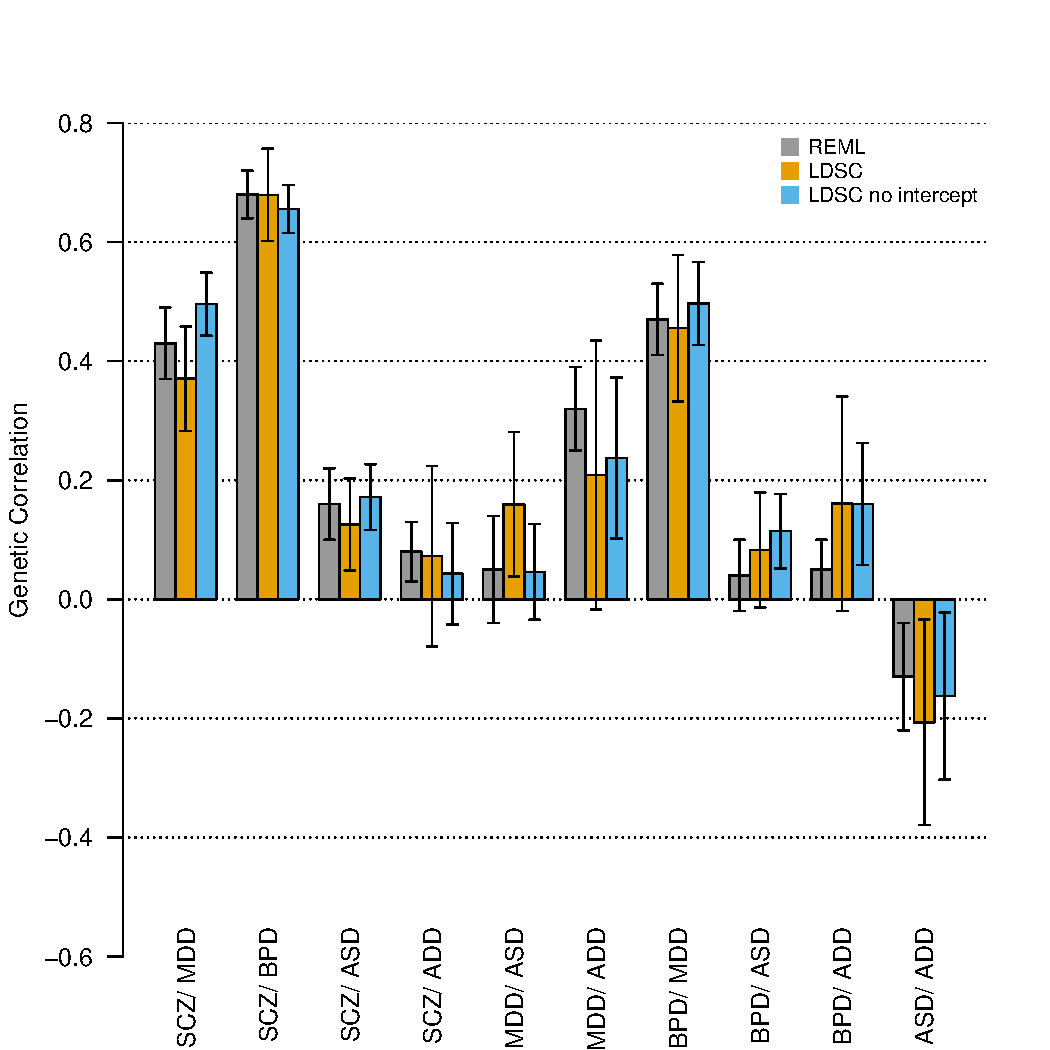
\includegraphics[scale=0.9]{figs/ldsc_vs_gcta.pdf}
\end{centering}
\caption{\label{Fig:Replication of PGC Cross-Disorder Results}\small{\textit{Replication of PGC Cross-Disorder Results.
This plot compares LD Score regression estimates of genetic correlation using the summary statistics from \cite{cross2013identification} (which were generated from approximately the same data as \cite{pgccdg2013}) to 
estimates obtained from REML in \cite{pgccdg2013}.
The horizontal axis indicates pairs of phenotypes, and the vertical axis indicates genetic correlation.
The error bars show standard errors.
Colors indicate different estimation procedures. Green is REML,
orange is LD Score with intercept and white is LD Score with constrained intercept.
The estimates of genetic correlation between psychiatric phenotypes in figure \ref{Fig:300 Gencors} use larger sample sizes;
this plot is intended primarily as a technical validation.
Abbreviations: 
ADD = attention deficit hyperactivity disorder;
ASD = autism spectrum disorder;
BPD = bipolar disorder;
MDD = major depressive disorder;
SCZ = schizophrenia.}}}
\end{figure}

\subsection*{Application to Summary Statistics From 25 Phenotypes}

We used LD Score regression to estimate genetic correlations among 25 phenotypes (URLs, Methods).
Genetic correlation estimates for all 300 pairwise combinations of the 25 traits are displayed in Figure \ref{Fig:300 Gencors}.
For clarity of presentation, 
the 25 phenotypes were restricted to contain only one phenotype from each cluster of highly correlated phenotypes (Methods).
Highly correlated educational, anthropometric, smoking, and insulin-related phenotypes that were excluded from Figure \ref{Fig:300 Gencors}
are displayed in Table \ref{edu} and Figures \ref{giant}, \ref{smoking} and \ref{insulin}, respectively.
References and sample sizes are displayed in Table \ref{N}.

% Figure 2 -- Genetic correlation heatmap with 25 traits
\begin{figure}[!ht]
\begin{centering}
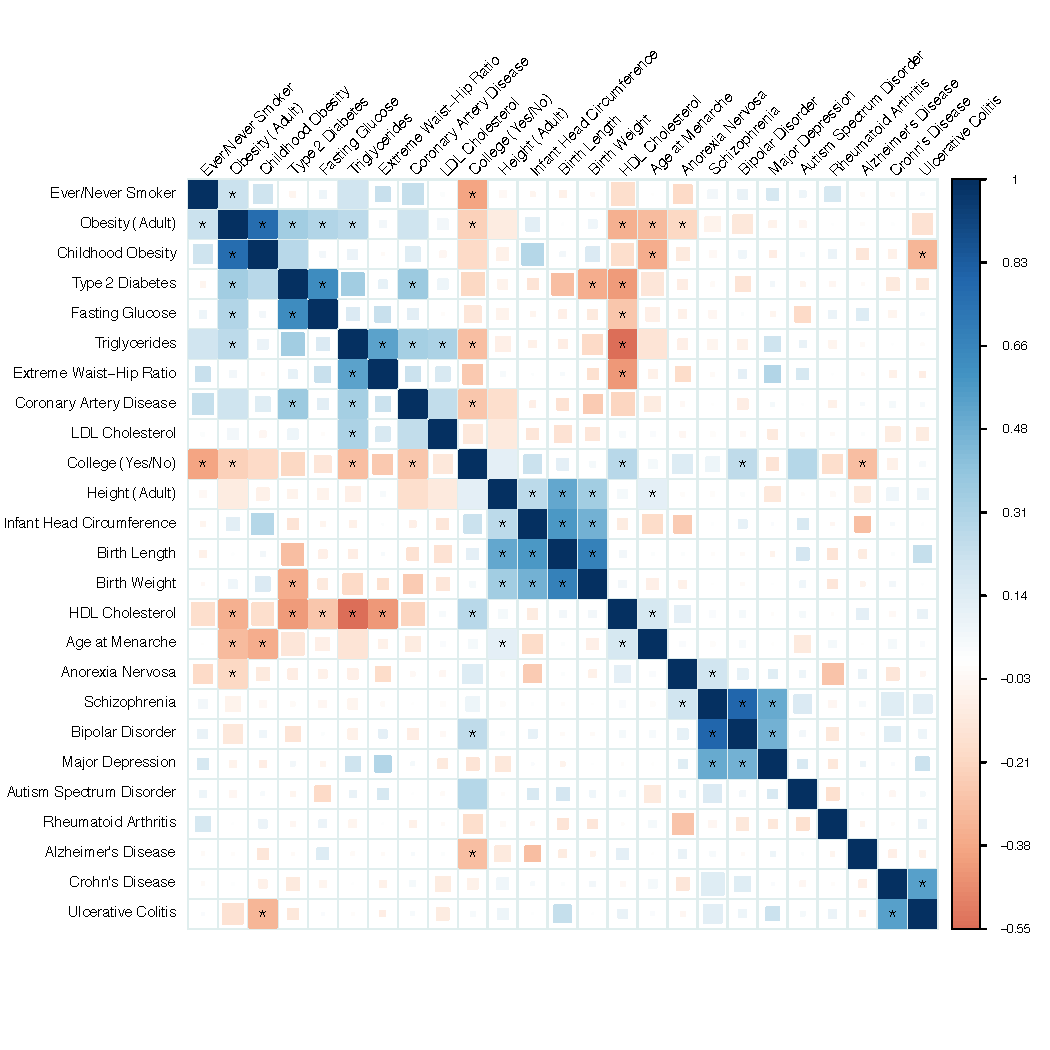
\includegraphics[scale=0.9]{figs/rg_heatmap.pdf}

\caption{         
\label{Fig:300 Gencors}
\small{\textit{Genetic Correlations among 25 Published GWAS.
Blue corresponds to positive genetic correlations; red corresponds to negative genetic correlation. 
Larger squares correspond to more significant $p$-values.
Genetic correlations that are different from zero at 1\% FDR are displayed as full-sized squares. 
Genetic correlations that are significantly different from zero at significance level 0.05 after Bonferroni correction for the 300 tests in this figure are given an asterisk. 
We display results that do not pass multiple testing correction as smaller squares in order to avoid the confusion that would result from whiting our positive controls that do not pass multiple testing correction because of small sample size.
This multiple testing correction is conservative, since the tests are not independent.}}}
\end{centering}
\end{figure}

% Results that are consistent with top SNP results or MR analyses 
For the majority of pairs of traits in Figure \ref{Fig:300 Gencors}, no GWAS-based genetic correlation estimate has been reported; 
however, many associations have been described in an \emph{ad-hoc} manner based off the observation of overlap among genome-wide significant loci.
Examples of genetic correlations that are consistent with overlap among top loci include the correlations between plasma lipids and cardiovascular disease \cite{do2013common}; age at onset of menarche and obesity \cite{perry2014parent}; type 2 diabetes, obesity, fasting glucose, plasma lipids and cardiovascular disease \cite{morris2012large}; birth weight, adult height and type 2 diabetes \cite{horikoshi2013new}; birth length, adult height and infant head circumference \cite{early2012genome, taal2012common}; and childhood obesity and adult obesity \cite{early2012genome}. 
For many of these pairs of traits, we can reject the null hypothesis of zero genetic correlation with overwhelming statistical
significance (\emph{e.g.,} $p<10^{-20}$ for age at onset of menarche and obesity).

% Table 1 -- interesting genetic correlation results highlighted in the main text
\begin{table}[h!]
\centering
\begin{tabular}{ l|llll}
 & Phenotype 1 & Phenotype 2 & $r_g$ (se) & $p$-value \\
\hline
\multirow{13}{*}{Epidemiological} 
& Age at Menarche & Height (Adult) & 0.11 (0.03) & $6\times10^{-5\ **}$  \\
& Age at Menarche & Type 2 Diabetes & -0.13 (0.04) & $3\times10^{-3}$  \\
& Age at Menarche & Triglycerides & -0.15 (0.04) & $1\times10^{-3\ *}$ \\
& Coronary Artery Disease & Age at Menarche &  -0.11 (0.05) & $4\times10^{-2}$ \\
& Coronary Artery Disease & College (Yes/No) & -0.278 (0.07) & $1\times10^{-4\ **}$ \\
& Coronary Artery Disease & Height (Adult) &  -0.17 (0.05) & $2\times10^{-4\ *}$\\
& Alzheimer's & College (Yes/No) & -0.30 (0.08) & $1\times10^{-4\ **}$ \\
& Bipolar Disorder & College (Yes/No) & 0.026 (0.064) & $6\times10^{-5\ **}$ \\
& Obesity (Adult) & College (Yes/No) & -0.23 (0.04) & $2\times10^{-8\ **}$\\
& Triglycerides & College (Yes/No) &-0.30 (0.04)&$5\times10^{-12\ **}$ \\
& Anorexia Nervosa & Obesity (Adult) & -0.20 (0.04) & $4\times10^{-6\ **}$ \\
& Ever/Never Smoker & College (Yes/No) & -0.39 (0.07) & $1\times10^{-9\ **}$ \\
& Ever/Never Smoker & Obesity (Adult) & 0.22 (0.05) & $7\times10^{-5\ **}$ \\
\hline
\multirow{3}{*}{Novel/Nonzero} 
& Autism Spectrum Disorder & College (Yes/No) & 0.28 (0.08) & $5\times10^{-4\ *}$\\
& Ulcerative Colitis & Childhood Obesity & -0.33 (0.08) & $3.9\times10^{-5\ **}$\\
& Anorexia Nervosa & Schizophrenia & 0.19 (0.04)  & $1.5\times10^{-5\ **}$ \\
\hline
\multirow{8}{*}{Novel/Zero} 
& Schizophrenia &Alzheimer's &  0.05 (0.05) & 0.58 \\
& Schizophrenia & Ever/Never Smoker & 0.03 (0.06) & 0.26 \\
& Schizophrenia & Triglycerides & -0.05 (0.04) & 0.21 \\
& Schizophrenia & LDL Cholesterol & -0.02 (0.03) & 0.64 \\
& Schizophrenia & HDL Cholesterol & 0.03 (0.04) & 0.50 \\
& Schizophrenia & Rheumatoid Arthritis & -0.05 (0.05) & 0.38 \\
& Crohn's Disease & Rheumatoid Arthritis & -0.02 (0.09) & 0.83 \\
& Ulcerative Colitis & Rheumatoid Arthritis & -0.09 (0.09) & 0.33 \\
\end{tabular}
\caption{
\small{\textit{\label{table:results}Genetic correlation estimates, standard errors and $p$-values for selected pairs of traits. Results are grouped into
 genetic correlations that are novel genetic results, but are consistent with established epidemiological associations (``Epidemiological''), novel genetic correlations (``Novel/Nonzero'') and interesting null results (``Novel/Zero''). 
 The $p$-values displayed are uncorrected $p$-values.
Results that pass multiple testing correction for the 300 tests in Figure \ref{Fig:300 Gencors} at 1\% FDR are given a single asterisk; results that pass Bonferroni correction at significance level 0.05 are given two asterisks.
For completeness, we present some genetic correlations that are directionally consistent with epidemiological associations but that do not pass multiple testing correction in our data. }}}
\end{table}

% Novel genetic results that are not novel epidemiological results
The first section of table \ref{table:results} lists genetic correlation results that are consistent with well-known epidemiological associations, 
but, as far as we are aware, have not previously been reported using genetic data.
Our estimates of the genetic correlation between age at onset of menarche and adult height \cite{onland2005age}, cardiovascular disease \cite{day2014} and type 2 diabetes \cite{day2014, elks2013age} are consistent with the epidemiological associations. 
Our estimate of a negative genetic correlation between AN and obesity (and a similar genetic correlation with BMI) is intriguing given that the most striking feature of anorexia nervosa is the ability to maintain dangerously low BMI \cite{american2013dsm} and suggests that similar genetic factors may influence normal variation in BMI as well as severely dysregulated BMI in psychiatric illness.
This result is consistent with our observation that BMI GWAS findings appear to primarily implicate neuronal, rather than metabolic, cell-types and epigenetic marks 
\cite{finucane2014partitioning}.
The negative genetic correlation between adult height and coronary artery disease agrees with a replicated epidemiological association  \cite{wang2011associations,hebert1993height,rich1995height}.
We observe several significant associations with the educational attainment phenotypes from
Rietveld \emph{et al.} \cite{rietveld2013gwas}.
We estimate a statistically significant negative genetic correlation between college and Alzheimer's disease, 
consistent with the epidemiological observation that low educational attainment is one of the largest risk factors for Alzheimer's
\cite{barnes2011projected, norton2014potential}. 
The positive genetic correlation between college and bipolar disorder is consistent with psychiatric literature showing that educational attainment and bipolar disorder status are positively correlated
\cite{maccabe2010excellent, tiihonen2005premorbid}, 
Our estimate of a negative genetic correlation between smoking and college is consistent with the epidemiological result that smoking is more prevalent among less-educated groups \cite{pierce1989trends}.
Finally, our estimates of genetic correlations among metabolic traits are consistent with the estimates obtained using REML in Vattikuti \emph{et al.}
\cite{vattikuti2012heritability} (Supplementary Table \ref{vattikuti}), and are directionally consistent with the recent Mendelian randomization results from Wuertz \emph{et al.} \cite{wuertz2014metabolic}.
In addition, our estimate of 0.57 (0.074) for the genetic correlation between Crohn's disease and ulcerative colitis is consistent
with the estimate of 0.62 (0.042) from Chen \emph{et al.} \cite{chen2014estimation}.


% Novel results
The second section of table \ref{table:results} lists results that are, to the best of our knowledge, new both to genetics and epidemiology.
First, we find a positive genetic correlation between anorexia nervosa and schizophrenia.
Comorbidity between eating and psychotic disorders has not been thoroughly investigated in the psychiatric literature \cite{striegel1999psychiatric,blinder2006psychiatric}, and our results raise the intriguing possibility of fundamental similarity between these classes of disease.
Second, we estimate a negative genetic correlation between ulcerative colitis and childhood obesity.
The relationship between premorbid BMI and ulcerative colitis is at present not well-understood,
and our results suggest that exploring this relationship may be a fruitful direction for further investigation. 
Third, we estimate a positive genetic correlation between autism spectrum disorder (ASD) and educational attainment,
which itself has very high genetic correlation with IQ \cite{deary2007intelligence, calvin2010sex, rietveld2013gwas}.
The ASD summary statistics were generated using a case-pseudocontrol study design, so this result cannot be explained by diagnostic biases, such as the tendency for the parents of children who receive a diagnosis of ASD to be better educated than the general population \cite{durkin2010socioeconomic}. 
The distribution of IQ among individuals with ASD has lower mean than the general population, but with heavy tails \cite{robinson2014autism} (\emph{i.e.,} an excess of individuals with extremely low and extremely high IQ).
In addition, there is evidence that the genetic architectures of high IQ and low IQ ASD are dissimilar \cite{samocha2014framework}.
We are unable to offer an explanation for this result, but propose that further exploration of this genetic correlation is an interesting direction for future research.

% Interesting null results
The third section of table \ref{table:results} lists several instances where the genetic correlation is close to zero with small standard error, in contrast to previous reports of epidemiological correlation or pleiotropy.
We estimate genetic correlations close to zero between schizophrenia and rheumatoid arthritis, schizophrenia and smoking, and schizophrenia and plasma lipids. The lack of genetic correlation between schizophrenia and rheumatoid arthritis is interesting because schizophrenia has been observed to be protective for rheumatoid arthritis \cite{silman2002epidemiology}.
The absence of genetic correlation between schizophrenia and smoking is notable because of the high prevalence of smoking among individuals with schizophrenia \cite{de2005meta}. 
Our estimate of zero genetic correlation between schizophrenia and plasma lipid levels or cardiovascular disease contrasts with earlier reports of extensive pleiotropy between schizophrenia and triglycerides \cite{andreassen2013improved2}. 
However, the observation from Andreassen, \emph{et al.} \cite{andreassen2013improved2} could potentially be explained the sensitivity of the method used in the original report to the properties of a few regions with high linkage disequilibrium, 
rather than trait biology (Table \ref{qq_tg}).
We estimate near-zero genetic correlation between Alzheimer's disease and schizophrenia. 
The genetic correlations between Alzheimers disease and the other four psychiatric traits (anorexia nervosa, bipolar, major depression, ASD) are also
close to zero, but with larger standard errors, due to smaller sample sizes.
This suggests that the genetic basis of Alzheimer's disease is distinct from psychiatric conditions. 
Last, we estimate near zero genetic correlation between rheumatoid arthritis and both Crohn's disease and ulcerative colitis. Although these immune diseases share a large number of associated loci \cite{cotsapas2011pervasive,farh2014genetic}, 
it is as often the case that an allele that is risk-increasing for one immune disease is protective for another as an allele is 
risk-increasing for two \cite{cotsapas2011pervasive}, consistent near-zero genetic correlation overall.
This is an example of pleiotropy without genetic correlation (Methods).
%%% Getting # of overlapping gwsig loci w/ concordant and discordant effects from Mark D

 
%%%%%%%%%%%%%%%%%%%%%%%%%%%%%%%%%%%%%%%%%%%%%%%%%%%%%%%%%%%%%%%
\section*{Discussion}\label{Discussion}
%%%%%%%%%%%%%%%%%%%%%%%%%%%%%%%%%%%%%%%%%%%%%%%%%%%%%%%%%%%%%%%\


% Summary of major findings
We have described a new method for estimating genetic correlation from GWAS summary statistics.
We applied our method to a large dataset of publicly available GWAS summary statistics, spanning 25 traits and more than 1.5 million phenotype-genotype pairs. 
We replicated many previously-reported GWAS-based genetic correlations, and confirm observations of overlap among genome-wide significant SNPs, 
Mendelian randomization results and known epidemiological associations, thus validating the utility of genetic correlation as an epidemiological tool.
In addition, we report several novel results that merit further analysis, including a positive genetic correlation between educational attainment and autism spectrum disorder
and a positive genetic correlation between anorexia nervosa and schizophrenia.

% Importance of findings 
This method is an advance for several reasons: 
it does not require individual genotypes, genome-wide significant SNPs or measuring all traits on all individuals;
it is not biased by sample overlap; 
and it is computationally trivial.  
Although it may be possible to extend existing methods such as LD-pruned polygenic scores to work on pairs of summary statistics, 
such methods would be biased by sample overlap, and would suffer from the disadvantage that LD-pruning results in loss of information.
These advantages allow estimation of genetic correlations between a much large set of pairs of phenotypes than was previously possible.

% Limitations of Genetic Correlation
In general, the difficulties in interpreting genetic correlation are similar to the difficulties in interpretation of Mendelian randomization.
Although genetic correlation is immune to environmental confounding, 
genetic correlation is still subject to genetic confounding, 
which is similar to the idea of confounding by pleiotropy from the Mendelian randomization literature (Methods).
This is best illustrated with an example. 
% Alkes suggested moving this example to the supplement in order to obtain a shorter discussion. I think it is a very important
% point, and prefer to leave it in the main text. Ben also seems keen to leave it in.
The negative genetic correlation between HDL and CAD in Figure \ref{Fig:300 Gencors} could result from a direct causal effect $\mathrm{HDL}\rightarrow\mathrm{CAD}$,
but could also result from non-causal shared genetic etiology, 
perhaps mediated by the genetic correlation of -0.55 between HDL and triglycerides (TG),
which is the explanation offered in \cite{do2013common, burgess2014using}. 
This scenario can be represented graphically as 
$\mathrm{HDL}\leftarrow\mathrm{G}\rightarrow\mathrm{TG}\rightarrow\mathrm{CAD}$, 
where $\mathrm{G}$ is the set of genetic variants with effects on both HDL and TG.
This diagram would result in a genetic correlation between HDL and CAD, because there is an unblocked path from HDL to CAD \cite{greenland1999causal}.
Extending genetic correlation to deal with multiple phenotypes that share causal loci 
(\emph{e.g.,} genetic correlation between HDL and CAD controlling for TG, 
analogous to \cite{do2013common,burgess2014using}) is an important direction for future work.

% Limitations of the Method
We note several limitations of the LD Score regression estimator of genetic correlation.
First, LD Score regression requires larger sample sizes than methods such as REML that use individual genotypes
in order to give estimates with acceptable standard error.
Second, LD Score regression is only currently applicable to studies that sample individuals from non-admixed populations
for which a sequenced reference panel (such as 1000 Genomes \cite{10002012integrated}) is available \cite{buliksullivan2014}.
Third, LD Score regression performs optimally when applied to traits with highly polygenic genetic architectures, such as 
psychiatric traits. 
At very large sample size and for less-polygenic traits,
analyzing only the significantly associated SNPs can sometimes be a more powerful strategy.
Developing methods that can make optimal use of both confidently associated large-effect SNPs and diffuse polygenic signal from thousands of small-effect SNPs is a direction for future research.
Fifth, although LD Score regression is not biased by oversampling of cases in case-control studies,
the results may nonetheless be biased by more subtle biases in ascertainment, such as misclassification of cases \cite{pgccdg2013}.

Despite these limitations, we believe that the LD Score regression estimator of genetic correlation will be a useful addition
to the epidemiological toolbox, since it allows for rapid screening for correlations among a diverse set of traits, without the 
need for measuring multiple traits on the same individuals or genome-wide significant SNPs.

%%% INSERT CONCLUSION HERE

\newpage
%%%%%%%%%%%%%%%%%%%%%%%%%%%%%%%%%%%%%%%%%%%%%%%%%%%%%%%%%%%%%%%
\section*{Methods}\label{Methods}
%%%%%%%%%%%%%%%%%%%%%%%%%%%%%%%%%%%%%%%%%%%%%%%%%%%%%%%%%%%%%%%

\subsection*{Definition of Genetic Covariance and Correlation}

Let $S$ denote a set of $M$ SNPs, 
let $X$ denote the random $M$-vector of additively (0-1-2) coded genotypes for the SNPs in $S$, 
and let $y_1$ and $y_2$ denote phenotypes $\beta := \mathrm{argmax}_{\alpha\in\R^M} \corr\left[y, X\alpha\right]^2$,
where the maximization is performed in the population (\emph{i.e.,} in the infinite data limit).
This is a projection, so uniqueness of $\beta$ is guaranteed as we remove SNPs that are linearly dependent (in the population). 
Then $h^2_S$, the heritability accounted for by SNPs in $S$, is defined $h^2_S(y_1) := \sum_j \beta_j^2$, and the genetic covariance among SNPs in $S$ is defined
$\rho_S(y_1,y_2) := \sum_{j\in S} \beta_j\gamma_j$.
It is more common to instead report genetic correlation, $r_S(y_1,y_2) := \rho_S(y_1,y_2)/\sqrt{h^2_S(y_1)h^2_S(y_2)}$, which lies in the interval [-1,1]. 
Following \cite{yang2010}, we use subscript $g$ (as in $h^2_g,\rho_g,r_g$) when the set of SNPs is 
genotyped and imputed SNPs in GWAS.

SNP genetic correlation (\emph{i.e.,} $S$ equals genotyped SNPs) is different from family study genetic correlation.
In a family study, the relationship matrix captures information about all genetic variation, 
not just common SNPs, so family studies estimate the total narrow-sense genetic correlation (\emph{i.e.,} $S$ equals all variants).
Unlike the relationship between SNP-heritability \cite{yang2010} and total narrow-sense heritability, 
for which we have the inequality $h^2_g \leq h^2$, 
no similar relationship holds between SNP genetic correlation and total narrow-sense genetic correlation.
For example, if $\beta$ and $\gamma$ are strongly correlated among common variants, but only weakly correlated among rare
variants, then the total narrow-sense genetic correlation will be less than the SNP genetic correlation.
Choice of the set of SNPs $S$ is discussed in the Supplementary Note.

Genetic correlation is (asymptotically) proportional to Mendelian randomization estimates.
Suppose we wish to estimate the effect $b$ of $y_1$ on $y_2$ using two-stage least squares (2SLS) \cite{angrist2008mostly} and a genetic instrument
 $g_i := \sum_{j\in S} X_{ij}\beta_j$, where $i$ indexes individuals
and $S$ is a set of SNPs. 
The 2SLS estimate is $\hat{b}_{2SLS}:=\T{g}y_2/\T{g}y_1$, and
$\E[\T{g}y_2]=\rho_S(y_1,y_2)$ and $\E[\T{g}y_1]=h^2_S(y_1)$.
Thus, $\lim_{N\to\infty} \hat{b}_{2SLS} = r_S(y_2,y_1)\sqrt{h^2_S(y_1) / h^2_S(y_2)}$.
If $S$ is the set of all SNPs, then this instrument has the (possibly undesirable) property of being symmetric in $y_1$ and $y_2$. This is discussed further in the Supplementary Note.

Genetic correlation is different from pleiotropy. 
Two traits have a pleiotropic relationship if many genetic variants have nonzero effects on both traits.
Genetic correlation is a stronger condition than pleiotropy:
to exhibit genetic correlation, it is not sufficient for two phenotypes to be influenced by overlapping sets of genetic variants, the directions of effects must also be consistently aligned across the genome.
Both quantities are informative: if two phenotypes are influenced by variants at the same loci or in the same pathways, 
this may indicate important shared biology, even if the direction of the effects do not align. 

%%%%%%%%%%%%%%%%%%%%%%%%%%%%%%%%%%%%%%%%%%%%%%%%%%%%%%%%%%%%%%%
\subsection*{Cross-Trait LD Score Regression} 
%%%%%%%%%%%%%%%%%%%%%%%%%%%%%%%%%%%%%%%%%%%%%%%%%%%%%%%%%%%%%%%

We estimate genetic covariance (technically $\pf$, see Supplementary Note) by regressing $z_{1j}z_{2j}$ against $\ell_j\sqrt{N_{1j}N_{2j}}$,
(where $N_{ij}$ is the sample size for SNP $j$ in study $i$) 
then multiplying the resulting slope by $M$, the number of SNPs in the reference panel with MAF between 5\% and 50\%.

If we know ahead of time that there is no sample overlap, we can constrain the intercept of this regression to zero (that is,
regression through the origin), which gives lower standard error. This can be accomplished with the \texttt{--no-intercept}
flag in \texttt{ldsc}.

%%%%%%%%%%%%%%%%%%%%%%%%%%%%%%%%%%%%%%%%%%%%%%%%%%%%%%%%%%%%%%%
\subsection*{Regression Weights} 
%%%%%%%%%%%%%%%%%%%%%%%%%%%%%%%%%%%%%%%%%%%%%%%%%%%%%%%%%%%%%%%

For heritability estimation, we use the LD Score regression weights derived in the 
Supplementary Note from \cite{buliksullivan2014}. 
If effect sizes for both phenotypes are drawn from a bivariate normal distribution, then
the optimal regression weights for genetic covariance estimation are 
\begin{equation}
\var[z_{1j}z_{2j} \,|\, \ell_j ] \propto
	\left( 
		\frac{N_1\hsqo\ell_j}{M} + 1
	\right) 
	\left(  
		\frac{N_2\hsqt\ell_j}{M} + 1
	\right) 
	+ 					
	2\left( 
		\dfrac{\sqrt{N_1N_2}\rho_g}{M}\ell_j + \dfrac{\rho N_s}{\sqrt{N_1N_2}}
	\right)^2
\end{equation}
(Supplementary Note). This quantity depends on both heritabilities, 
the genetic covariance and the number of overlapping samples,
which are not known a priori, so it is necessary to estimate them from the data.
Linear regression with weights estimated from the data is called feasible generalized least squares (FGLS) \cite{angrist2008mostly}. 
We run a first LD Score regression weighted with weights computed using the heritability estimates from the single-phenotype LD Score regressions,
$N_s$ set to zero, and $\rho_g$ estimated with the aggregate estimator 
$\hat{\rho}_{g, agg} := (\lbar\sqrt{N_1N_2})^{-1}\sum_j z_{1j}z_{2j},$
where $\lbar$ denotes the mean LD Score among SNPs included in the regression.
We then update the weights using the estimates of $\rho_g$ and $\rho N_s$ obtained from the first LD Score regression and use the updated weights for the second and final LD Score regression.
In addition, we weight by $1/\ell_j$ (where $\ell_j$ here denotes LD Score with the sum taken over SNPs included in the regression) in order to downweight SNPs that are overcounted. 
This is a heuristic: the optimal approach would be to weight by the inverse covariance matrix of $\chi^2$-statistics, but this matrix is difficult to compute.

%%%%%%%%%%%%%%%%%%%%%%%%%%%%%%%%%%%%%%%%%%%%%%%%%%%%%%%%%%%%%%%
\subsection*{Assessment of Statistical Significance via Block Jackknife}
%%%%%%%%%%%%%%%%%%%%%%%%%%%%%%%%%%%%%%%%%%%%%%%%%%%%%%%%%%%%%%%

Under a polygenic model, the $\chi^2$-statistics and $Z$-score products for SNPs in LD are correlated, so 
 the usual estimator of the regression standard error, which assumes that all data points are independent, will be biased downwards. 
Therefore, we use a block jackknife over blocks of adjacent SNPs in order to obtain a correlation-robust standard error. 
The default setting in \texttt{ldsc} is 200 blocks per genome, which can be adjusted with the \texttt{--num-blocks} flag.
This is the same procedure used in \cite{buliksullivan2014}, and gives accurate standard errors in simulations (Table \ref{se_sim}).
We also obtain a standard error for the genetic correlation by using a ratio block jackknife over SNPs.

%%%%%%%%%%%%%%%%%%%%%%%%%%%%%%%%%%%%%%%%%%%%%%%%%%%%%%%%%%%%%%%
\subsection*{Computational Complexity}
%%%%%%%%%%%%%%%%%%%%%%%%%%%%%%%%%%%%%%%%%%%%%%%%%%%%%%%%%%%%%%%

If $N$ denotes sample size and $M$ denotes the number of SNPs, then LD Score regression takes
$\mathscr{O}(MN)$ time for computing summary statistics and $\mathscr{O}(M)$ time for the regression. 
Estimating LD Scores takes $\mathscr{O}(MN)$ time, though $N$ for estimating LD Scores does not need to as large as $N$
for GWAS; for instance, we use $N=378$ Europeans from 1000 Genomes for estimating LD Score. 
In addition, LD Scores only need to be computed once, and can then be applied to many pairs of phenotypes.
For comparison, REML takes time $\mathscr{O}(MN^2)$ for computing the genetic relatedness matrix (GRM)
and $\mathscr{O}(N^3)$ time for maximizing the likelihood.

Practically, estimating LD Scores takes about an hour parallelized over chromosomes, and
LD Score regression takes about 15 seconds for each pair of phenotypes on a standard 2014 MacBook Air with 1.7 GhZ Intel Core i7 processor.

%%%%%%%%%%%%%%%%%%%%%%%%%%%%%%%%%%%%%%%%%%%%%%%%%%%%%%%%%%%%%%%
\subsection*{Summary Statistic Datasets}\label{datasets}
%%%%%%%%%%%%%%%%%%%%%%%%%%%%%%%%%%%%%%%%%%%%%%%%%%%%%%%%%%%%%%%

We selected traits for inclusion in the main text via the following procedure:

\begin{enumerate}
\itemsep-0.1em
\item Begin with all publicly available non-sex-stratified European-only summary statistics that provide signed summary statistics, are imputed to at least HapMap 2 and do not include heritable covariates.
\item Remove all traits with heritability $Z$-score below 4, based on the observation that genetic correlations for traits with heritability $Z$-score below 4 are generally too noisy to interpret.
\item Prune sets of highly correlated phenotypes (\emph{e.g.,} obesity classes 1-3, or the several glucose and insulin measures from the MAGIC consortium) by picking the trait from each cluster with the highest heritability heritability $Z$-score (traits pruned in this step are displayed in the supplementary figures).

\end{enumerate}

We then applied the following filters (encoded in the script \texttt{sumstats\_to\_chisq.py} included with our \texttt{ldsc} software package) to the summary statistics:
\begin{enumerate}
\itemsep-0.1em
\item For studies that provide a measure of imputation quality (\emph{e.g.,} INFO score), filter to INFO greater than 0.9.
\item For studies that provide sample MAF, filter to sample MAF above 1\%.
\item In order to restrict to well-imputed SNPs in studies that do not provide a measure of imputation quality, filter to HapMap3 \cite{international2010integrating} SNPs with HapMap3 MAF above 1\%, which tend to be well-imputed in most studies. This 
step should be skipped if INFO scores are available for all studies.
\item If sample size varies from SNP to SNP, remove SNPs with effective sample size less than two thirds of the the 90th percentile of sample size.
\item Remove indels and structural variants.
\item Remove strand-ambiguous SNPs.
\item Remove SNPs whose alleles do not match the alleles reported in 1000 Genomes.
\item Because the presence of outliers can increase the standard error of the LD Score regression estimates, we also removed
 SNPs with extremely large effect sizes ($\chi^2 > 80$, as in \cite{buliksullivan2014}).
\end{enumerate}

If the summary statistics have been GC corrected at any point in the data-generating process, then the heritability and genetic covariance estimates
will be biased downwards. The bias in the numerator and denominator of genetic correlation will precisely cancel, so genetic correlation estimates are not affected by GC correction. 
The majority of the datasets analyzed in this paper were GC corrected at least once, which is why we do not report genetic covariance and heritability.

Data on Alzheimer's disease were obtained from the following source:

\begin{quotation}
    \textit{\small{International Genomics of Alzheimer's Project (IGAP) is a large two-stage study based upon genome-wide association studies (GWAS) on individuals of European ancestry. 
    In stage 1, IGAP used genotyped and imputed data on 7,055,881 single nucleotide polymorphisms (SNPs) to meta-analyze four previously-published GWAS datasets consisting of 17,008 Alzheimer's disease cases and 37,154 controls 
    (The European Alzheimer's Disease Initiative, EADI; the Alzheimer Disease Genetics Consortium, ADGC; The Cohorts for Heart and Aging Research in Genomic Epidemiology consortium, CHARGE; The Genetic and Environmental Risk in AD consortium, GERAD). 
    In stage 2, 11,632 SNPs were genotyped and tested for association in an independent set of 8,572 Alzheimer's disease cases and 11,312 controls. 
    Finally, a meta-analysis was performed combining results from stages 1 and 2.}}
\end{quotation}
We only used stage 1 data for LD Score regression.

\newpage

%%%%%%%%%%%%%%%%%%%%%%%%%%%%%%%%%%%%%%%%%%%%%%%%%%%%%%%%%%%%%%%
\section*{URLs}\label{URLs}
%%%%%%%%%%%%%%%%%%%%%%%%%%%%%%%%%%%%%%%%%%%%%%%%%%%%%%%%%%%%%%%
\begin{enumerate}
\itemsep-0.1em

	\item \texttt{ldsc} software:\\ 
		\texttt{github.com/bulik/ldsc}
		
	\item This paper:\\
		\texttt{github.com/bulik/gencor\_tex}
		
	\item PGC (psychiatric) summary statistics:\\ 
		\texttt{www.med.unc.edu/pgc/downloads}
		
	\item GIANT (anthopometric) summary statistics: \\
		\texttt{www.broadinstitute.org/collaboration/giant/index.php/GIANT\_consortium\_data\_files}
	\item EGG (Early Growth Genetics) summary statistics:\\
		\texttt{www.egg-consortium.org/}
	
	\item MAGIC (insulin, glucose) summary statistics: \\
		\texttt{www.magicinvestigators.org/downloads/}
		
	\item CARDIoGRAM (coronary artery disease) summary statistics:\\	
		\texttt{www.cardiogramplusc4d.org}
	
	\item DIAGRAM (T2D) summary statistics:\\
		\texttt{www.diagram-consortium.org}
		
	\item Rheumatoid Arthritis summary statistics:\\
		\texttt{www.broadinstitute.org/ftp/pub/rheumatoid\_arthritis/Stahl\_etal\_2010NG/}
	
	\item IGAP (Alzheimers) summary statistics:\\
		\texttt{www.pasteur-lille.fr/en/recherche/u744/igap/igap\_download.php}

	\item IIBDGC (inflammatory bowel disease) summary statistics:\\
		\texttt{www.ibdgenetics.org/downloads.html}\\
		We used a newer version of these data with 1000 Genomes imputation.

	\item Plasma Lipid summary statistics:\\
		\texttt{www.broadinstitute.org/mpg/pubs/lipids2010/}
	
	\item Educational Attainment summary statistics:\\
		\texttt{www.ssgac.org/}
	
	\item Beans:\\
		\texttt{www.barismo.com}\\
		\texttt{www.bluebottlecoffee.com}
\end{enumerate}

\newpage
%%%%%%%%%%%%%%%%%%%%%%%%%%%%%%%%%%%%%%%%%%%%%%%%%%%%%%%%%%%%%%%
\section*{Acknowledgements}\label{Acknowledgements}
%%%%%%%%%%%%%%%%%%%%%%%%%%%%%%%%%%%%%%%%%%%%%%%%%%%%%%%%%%%%%%%

We would like to thank P. Sullivan, C. Bulik and S. Caldwell for helpful discussion. This work was supported by NIH grants R01 MH101244  (ALP), R03 CA173785 (HKF) and by the Fannie and John Hertz Foundation (HKF). The coffee that Brendan drank while writing this paper was roasted by Barismo in Arlington, MA and Blue Bottle Coffee in Oakland, CA. 

Data on anorexia nervosa were obtained by funding  from the WTCCC3 WT088827/Z/09 titled ``A genome-wide association study of anorexia nervosa''.

Data on glycaemic traits have been contributed by MAGIC investigators and have been downloaded from www.magicinvestigators.org.

Data on coronary artery disease / myocardial infarction have been contributed by CARDIoGRAMplusC4D investigators and have been downloaded from 
\texttt{www.CARDIOGRAMPLUSC4D.ORG}

We thank the International Genomics of Alzheimer's Project (IGAP) for providing summary results data for these analyses. The investigators within IGAP contributed to the design and implementation of IGAP and/or provided data but did not participate in analysis or writing of this report. IGAP was made possible by the generous participation of the control subjects, the patients, and their families. The i-Select chips was funded by the French National Foundation on Alzheimer's disease and related disorders. EADI was supported by the LABEX (laboratory of excellence program investment for the future) DISTALZ grant, Inserm, Institut Pasteur de Lille, Universit� de Lille 2 and the Lille University Hospital. GERAD was supported by the Medical Research Council (Grant 503480), Alzheimer's Research UK (Grant 503176), the Wellcome Trust (Grant 082604/2/07/Z) and German Federal Ministry of Education and Research (BMBF): Competence Network Dementia (CND) grant 01GI0102, 01GI0711, 01GI0420. CHARGE was partly supported by the NIH/NIA grant R01 AG033193 and the NIA AG081220 and AGES contract N01-AG-12100, the NHLBI grant R01 HL105756, the Icelandic Heart Association, and the Erasmus Medical Center and Erasmus University. ADGC was supported by the NIH/NIA grants: U01 AG032984, U24 AG021886, U01 AG016976, and the Alzheimer's Association grant ADGC-10-196728.


%%%%%%%%%%%%%%%%%%%%%%%%%%%%%%%%%%%%%%%%%%%%%%%%%%%%%%%%%%%%%%%
\section*{Author Contributions}\label{author_contribs}
%%%%%%%%%%%%%%%%%%%%%%%%%%%%%%%%%%%%%%%%%%%%%%%%%%%%%%%%%%%%%%%


MJD provided reagents
BMN and ALP provided reagents
CL, ER, VA, JP and FD aided in the interpretation of results.
JP and FD provided data.
The caffeine molecule is responsible for all that is good about this manuscript.
BBS and HKF are responsible for the rest.
All authors revised and approved the final manuscript.


%%%%%%%%%%%%%%%%%%%%%%%%%%%%%%%%%%%%%%%%%%%%%%%%%%%%%%%%%%%%%%%
\section*{Competing Financial Interests}
%%%%%%%%%%%%%%%%%%%%%%%%%%%%%%%%%%%%%%%%%%%%%%%%%%%%%%%%%%%%%%%

Unfortunately, we have no financial conflicts of interest to declare.

\newpage
\bibliographystyle{unsrt}
\bibliography{gencor}
\beginsupplement
\newpage
%%%%%%%%%%%%%%%%%%%%%%%%%%%%%%%%%%%%%%%%%%%%%%%%%%%%%%%%%%%%%%%
\section*{Supplementary Note}
%%%%%%%%%%%%%%%%%%%%%%%%%%%%%%%%%%%%%%%%%%%%%%%%%%%%%%%%%%%%%%%


\subsection*{Flavors of Genetic Correlation}

\subsection*{Quantitative Traits}
Suppose we sample two cohorts for two phenotypes,
$y_1$ and $y_2$,
with sample sizes $N_1$ and $N_2$,
such that $N_s$ individuals are shared between cohorts and phenotyped for both traits.
We model phenotypes as generated by the equations $y_1 = Y\beta + \delta$,
and $y_2 = Z\gamma + \epsilon$,
where $Y$ and $Z$ are matrices of genotypes normalized to mean zero and variance one\footnote{
We ignore the distinction between normalizing and centering in the population and in the sample, 
since this introduces only $\mathscr{O}(1/N)$ error.},
with dimensions $N_1\times M$ and $N_2\times M$, respectively; 
$\beta$ and $\gamma$ are $M\times 1$ vectors of per-normalized genotype effect sizes,
and $\delta$ and $\epsilon$ are vectors of environmental or non-additive genetic effects,
with dimensions $N_1\times 1$ and $N_2\times 1$, respectively.
In this model, $Y$ and $Z$ are unobserved matrices of all SNPs, including SNPs that are not genotyped.

We model all of $Y, Z, \beta, \gamma, \delta $ and $\epsilon$ as random variables.
Suppose that $(\beta, \gamma)$ has mean zero and covariance matrix\
\begin{equation*} 
	\var[(\beta, \gamma)] = \frac{1}{M}
		\left( \begin{array}{cc}
		\hsqo I & \gencov I\\
		\gencov I& \hsqt  I
	\end{array} \right),
\end{equation*}
and $(\delta, \epsilon)$ has mean zero and covariance matrix
\begin{equation*}
	\var[(\delta, \epsilon)] = 
		\left( \begin{array}{cc}
		(1-\hsqo) I & \envcov I\\
		\envcov I& (1-\hsqt) I
	\end{array} \right).
\end{equation*}
Finally, suppose that there are $N_s$ individuals who appear in both $Y$ and $Z$, and that the 
genotypes from all unique individuals are \emph{i.i.d.} draw from a distribution with covariance matrix $R$
(\emph{i.e.,} $r$ is an LD matrix with $r_{jk} = \E[Y_{ij}Y_{ik}]$.
Let $\rho := \gencov + \envcov$ denote the covariance between $y_1$ and $y_2$,
which is also the correlation between $y_1$ and $y_2$, since both have variance one.

The assumption that all $\beta$ is drawn with equal variance for all SNPs hides an implicit assumption that 
rare SNPs have larger per-allele effect sizes than common SNPs. 
As discussed in the simulations section of the main text and in our earlier work \cite{buliksullivan2014}, LD Score regression is robust to moderate violations of this assumption, though it may break down in extreme
cases, for instance if all causal variants are rare.
In situations where a different model for the variance of $\beta$ is more appropriate, all proofs in this note go through
with LD Score replaced by weighted LD Scores, $\ell_j = \sum_k \var[\beta_j]r^2_{jk}$.

\begin{prop} Under this model, the expected genetic covariance between phenotypes is $\gencov$, justifying our use of the notation $\gencov$.
\end{prop}
\begin{proof} Let $X$ denote an $1\times M$ vector of normalized, centered genotypes for an arbitrary individual. 
Under the model, the additive genetic component of $y_1$ for this individual is $\sum_jX_{ij}\beta_j$,
and the additive genetic component of $y_2$ for this individual is $\sum_jX_{ij}\gamma_j$.
Thus, the genetic covariance between $y_1$ and $y_2$ is 
\begin{align*}
	\cov\left[\sum_j X_j\beta_j,\sum_j X_j\gamma_j\right] &= 
		\E\left[\left(\sum_j X_j\beta_j\right)\left(\sum_j X_j\gamma_j\right)\right]\\
		&= \sum_j \sum_k \E[X_jX_k\beta_j\gamma_k]\\
		&= \sum_j \E[X_j^2\beta_j\gamma_j]\\
		&= \sum_j \E[X_j^2]\E[\beta_j\gamma_j]\\
		&= \rho_g.
\end{align*}
\end{proof}

\label{supp_condexp_qt}
Suppose we directly genotype SNP $j$. 
We compute $Z$-scores $z_{1j}:= \T{Y}_jy_1/\sqrt{N_1}$ and $z_{2j}:= \T{Y}_jy_1/\sqrt{N_2}$  from linear regression.
\begin{prop} 
Let $j$ denote a genotyped SNP. Under the model described above, 
\begin{equation}
	\E[z_{1j}z_{2j}] = \frac{\sqrt{N_1N_2}\gencov}{M}\ell_j  + \frac{N_s\rho}{\sqrt{N_1N_2}}.
\end{equation}
\end{prop}

\begin{proof} By the law of total expectation, 
$$\E[z_{1j}z_{2j}] = \E[ \E[z_{1j}z_{2j} \,|\, Y, Z ] ]$$
\noindent
First,
\begin{align*}
	\E[z_{1j}z_{2j}\,|\,Y,Z] &= \frac{1}{\sqrt{N_1N_2}}\E[\T{Y}_jy_1\T{y_2}Z_j]   \\
       		&= \frac{1}{\sqrt{N_1N_2}}\T{Y}_j\E[{(Y\beta+\delta)}(Z\gamma+\epsilon)]Z_j\\
        		&= \frac{1}{\sqrt{N_1N_2}}\T{Y}_j\left(Y\E[\beta\T{\gamma}]Z + \E[\T{\delta}\epsilon]\right)Z_j\\
        		&= \frac{1}{\sqrt{N_1N_2}}\left( \frac{\gencov}{M} \T{Y}_jY\T{Z}_jZ  + \envcov\T{Y}_jZ_j  \right).
\end{align*}
\noindent
To remove the conditioning on $Y$ and $Z$, we compute 
\begin{equation*}
\frac{1}{\sqrt{N_1N_2}}\E[\T{Y}_jZ_j ] = \frac{N_s}{\sqrt{N_1N_2}},
\end{equation*}
and 
\begin{equation*}
\frac{1}{\sqrt{N_1N_2}}\E[\T{Y}_jY\T{Z}_jZ] = \ell_j + \frac{MN_s}{\sqrt{N_1N_2}}.
\end{equation*}
Thus, 
\begin{align*}
	\E[z_{1j}z_{2j}] 
&= 
	\frac{\sqrt{N_1N_2}\gencov}{M}\ell_j  + \frac{N_s\left(\rho_g + \rho_e\right)}{\sqrt{N_1N_2}}\\
&=
	\frac{\sqrt{N_1N_2}\gencov}{M}\ell_j  + \frac{N_s\rho}{\sqrt{N_1N_2}}.
\end{align*}
Note that if study 1 and study 2 are the same study, then $N_1=N_2=N_s$, $\rho_g=h^2_g$, and this 
reduces to the LD Score regression equation for a single trait from \cite{buliksullivan2014}.
\end{proof}

%%%%%%%%%%%%%%%%%%%%%%%%%%%%%%%%%%%%%%%%%%%%%%%%%%%%%%%%%%%%%%%
\subsection*{Regression Weights}
%%%%%%%%%%%%%%%%%%%%%%%%%%%%%%%%%%%%%%%%%%%%%%%%%%%%%%%%%%%%%%%

We can improve the efficiency of the LD Score regression by computing the conditional variance 
$\var[\bhat\chat \,|\,\ell_j]$
and weighting the regression by the reciprocal of this variance. 
In order to compute this conditional variance, 
we need an additional distributional assumption.
Therefore we derive the conditional variance function for the case where 
 $Z$-scores follow a multivariate normal distribution\footnote{
For instance, it is sufficient but not necessary to assume that $\beta$, $\gamma$, $\delta$ and $\epsilon$ are multivariate normal, 
and that $N_1$ and $N_2$ are sufficiently large that we can invoke the central limit theorem. 
More generally, the phenotypes will be approximately normal if $\delta$ and $\epsilon$ are normal 
and if $\beta$ and $\gamma$ are reasonably polygenic.
If there are few casual SNPs, then the conditional variance may be larger.}.

If phenotypes are normally distributed, then by the central limit theorem,
$\bhat$ and $\chat$ are approximately distributed as bivariate normal with expectation zero. 
Then, from a standard formula for double second moments of the bivariate normal distribution
\begin{align}
    \var[\bhat_j\chat_j\cond\ell_j] 
&= 
	\E[\bhat^2\chat^2]\nonumber\\
&=  
	\var[\bhat]\var[\chat]
	+
	2\E[\bhat\chat]^2\nonumber\\
&= 
	\left( 
		\frac{\hsqo\ell_j}{M} 
		+ 
		\frac{1}{N_1} 
	\right) \left(  
		\frac{\hsqt\ell_j}{M} 
		+ 
		\frac{1}{N_2}
	\right) 
	+ 					
	2\left( 
		\frac{\gencov\ell_j}{M} 
		+ 
		\frac{\rho N_s}{N_1N_2} 
	\right)^2.
\end{align}

Note that we only assume normality in order to compute regression weights.
If (quantitative) phenotypes are not normally distributed,
this will not affect the expectation of the LD Score regression estimates; however, in this case LD Score regression may be inefficient, because the regression weights will be suboptimal.

\subsection*{Liability Threshold Model}

In the liability threshold model, binary traits are determined by an unobserved continuous liability $\psi$ generated following the usual model for quantitative traits: $\psi_i = \sum_j X_{ij}\beta_j + \epsilon_i$.
The observed binary phenotype is then has population prevalence $K$, 
and is generated from the unobserved liability via the liability threshold model: $y_i := \ind[\psi_i > \tau]$,
where $\tau$ denotes the liability threshold.
If $\psi$ is normally distributed, then setting $\tau:=\Phi^{-1}(1-K)$ (where $\Phi$ denotes the cdf of the standard normal distribution) yields a population prevalence of $K$.

For phenotypes generated according to the liability threshold model, we can estimate not only the heritability of the observed
phenotype (genetic covariance between the observed phenotype and other phenotypes), but also the heritability of the 
unobserved liability (genetic covariance between unobserved liability and other phenotypes).

Note that the liability threshold construction is surprisingly general. 
If $y$ is a binary phenotype, then we can define a normally distributed liability for $y$ by defining
$\psi_i$ to be a random draw from a normal distribution truncated at the left by $\tau$ if $y_i=1$ and 
truncated at the right by $\tau$ if $y_i=0$.
Therefore, we prefer to think of liability scale heritability as a useful way to compare the heritabilities of binary phenotypes
with different prevalences, rather than a quantity that is only meaningful if one is willing to make strong assumptions 
about the data generating process.

In this section, we derive population case and control allele frequencies 
$p_{cas,j} = \prob[G_{ij}=1\cond y_i=1]$ and $p_{con,j} = \prob[G_{ij}=1\cond y_i=0]$ in terms of the heritability of liability generated by a polygenic model,
where $G_{ij}$ denotes an un-normalized genotype (note that since we are only modeling additive effects and we are willing 
to assume Hardy-Weinberg equilibrium, we lose nothing and simplify notation by dealing with haploid genotypes).

\begin{prop}
Suppose unobserved liabilities $\psi, \varphi$ for traits $y_1,y_2$ with thresholds $\tau_1,\tau_2$ corresponding to prevalences $K_1,K_2$ are generated according to the usual polygenic model for quantitative traits, i.e.,
$\psi_i=\sum_j X_{ij}\beta_j+\delta$, $\varphi_i=\sum_j X_{ij}\gamma_j+\epsilon$, with $X$ random with a given LD matrix,
\begin{equation*} 
	\var[(\beta, \gamma)] = \frac{1}{M}
		\left( \begin{array}{cc}
		\hsqo I & \gencov I\\
		\gencov I& \hsqt  I
	\end{array} \right),
\end{equation*}
and
\begin{equation*}
	\var[(\delta, \epsilon)] = 
		\left( \begin{array}{cc}
		(1-\hsqo) I & \envcov I\\
		\envcov I& (1-\hsqt) I
	\end{array} \right).
\end{equation*}
Let $\zeta_j$ and $\xi_j$ denote the marginal effect size of $j$ on $\psi$ and $\varphi$, and let $p_{cas,kj}:=\prob[G_{ij}=1\cond y_{ik}=1]$ for $k=1,2$. Then
\begin{align*}
	\E[p_{cas,1j}] = p_j,\\
	\E[p_{cas,2j}] = p_j, \\
	\var[p_{cas,1j}] = \dfrac{p_j^2\phi(\tau_1)^2h^2_1}{MK_1^2}\ell_j, \\
	\var[p_{cas,2j}] = \dfrac{p_j^2\phi(\tau_2)^2h^2_2}{MK_2^2}\ell_j,\\
	\cov[p_{cas,1j},p_{cas,j}] = \dfrac{p_j^2\phi(\tau_1)\phi(\tau_2)\rho_g}{MK_1K_2}\ell_j.
\end{align*}
Note that these terms are different from the usual expressions for conversion from observed to liability scale, because we have not
yet accounted for ascertainment. We account for ascertainment in the next section.
\end{prop}
\begin{proof}
This proof is accomplished in two steps.
First, we compute allele frequencies conditional on the marginal effects on liability. 
To do this, we reverse the conditional probability using Bayes' theorem, 
which reduces the problem to a series of [Taylor approximations to] gaussian integrals. 
Second, we remove the conditioning on the marginal effects on liability and use the results of the previous section (on quantitative traits) to express the expectations of the allele frequencies
in terms of $h^2_1,h^2_2,\rho_g$ and $\ell_j$.

To begin, assume that the marginal effects $\zeta_j$ and $\xi_j$ are fixed.
By Bayes' theorem, 
\begin{align*}
	\prob[G_{ij}=1\cond y_{i1}=1,\zeta_j]
&=
	\dfrac{\prob[y_{i1}=1\cond G_{ij}=1,\zeta_j]\prob[G_{ij}=1]}{\prob[y_{i1}=1]}\\
&=
	\dfrac{p_j}{K_1}\prob[y_{i1}=1\cond G_{ij}=1,\zeta_j]\\
&=
	\dfrac{p_j}{K_1}\prob[\psi_i>\tau_1\cond G_{ij}=1,\zeta_j].
\end{align*}

The distribution of $\psi$ conditional on $\zeta_j$ and $G_{ij}=1$ is 
$\psi\cond\zeta_j,G_{ij}=1 = N(\zeta_j, 1-\zeta_j^2)\approx N(\zeta_j, 1)$ (where the approximation holds when $\zeta_j^2$ is small, \emph{i.e.,} when the marginal heritability explained by $j$ is small, which is the typical case in GWAS).
Thus $\prob[\psi_i>\tau_1\cond G_{ij}=1]$ is simply a Gaussian integral.
Because we wish to obtain a closed-form expression for the variance of $\prob[\psi_i>\tau_1\cond G_{ij}=1,\zeta_j]$ over random $\zeta_j$, we approximate this probability with a first-order Taylor expansion around $\tau_1$:
\begin{align*}
	\prob[\psi_i>\tau_1\cond G_{ij}=1,\zeta_j]
&=
	1-\Phi(\tau_1-\zeta_j)\\
&\approx
	K_1 + \phi(\tau_1)\zeta_j,
\end{align*}
where $\Phi,\phi$ denote the cdf and density of the standard normal distribution. Thus,
\begin{align}\label{condprob}
	\prob[G_{ij}=1\cond y_{i1}=1,\zeta_j]
&=
	p_j\left(1+\dfrac{\phi(\tau_1)\zeta_j}{K_1}\right).
\end{align}
An similar result holds for trait 2, replacing $\zeta$ with $\xi$ and subscript 1 with subscript 2.

We have written the probabilities in question in terms of constants and marginal effects on liability.
Since liability is simply a quantitative trait, the means, variances, and covariances of the marginal effects on liability
are described by the LD Score regression equation from the section on quantitative traits.
Precisely, $\E[\xi_j]=\E[\zeta_j] = 0$, $\var[\xi_j]=\hsqo\ell_j/M$, $\var[\zeta_j]=\hsqt\ell_j/M$ and $\cov[\zeta_j,\xi_j]=\rho_g\ell_j/M$.
Thus it follows from equation \ref{condprob} that first, $\E[p_{cas,1j}]=\E[p_{cas,2j}]=p_j$, second
\begin{align*}
	\var[p_{cas,1j}]
&=
	\var[p_j + p_j\phi(\tau_1)\zeta_j/K_1]\\
&=
	\dfrac{p_j^2\phi(\tau_1)^2h^2_1}{MK_1^2}\ell_j,
\end{align*}
(and similarly for trait two); and last
\begin{align*}
	\cov[p_{cas,1j},p_{cas,2j}]
&=
	\cov[p_j + p_j\phi(\tau_1)\zeta_j/K_1,p_j + p_j\phi(\tau_2)\xi_j/K_2]\\
&=
	\dfrac{p_j^2\phi(\tau_1)\phi(\tau_2)\rho_g}{MK_1K_2}\ell_j.
\end{align*} 
\end{proof}


\subsection*{Ascertained Studies of Liability Threshold Traits}

In this section, we derive an analogous LD Score regression equation for ascertained case/control studies.
The key elements of this derivation are (1) deriving the relationship between observed and liability scale heritability and genetic
covariance and (2) showing that out-of-sample LD from a non-ascertained reference panel is still a good approximation to
LD in an ascertained sample, even though oversampling of cases induces long-range LD between risk alleles.
The definitions of heritability and genetic covariance provided in the main text apply to binary traits, though we also 
discuss a new parameter, the liability scale heritability, which is a convenient scale for comparing the heritabilities of binary traits 
with different prevalences.

We keep the same notation from the previous section, except here $y_1$ and $y_2$ are binary phenotypes. 
In addition, let $P_i$ denote the sample prevalence of $y_i$ in study $i$ for $i=1,2$, and $K_i$ denote the population prevalence.

We compute $z$-scores
$Z_j := 
\frac
	{\sqrt{NP(1-P)}(\hat{p}_{cas} - \hat{p}_{con})} 
	{\sqrt{\hat{p}_j(1-\hat{p}_j)}},
$
where $\hat{p}_j$ denotes allele frequency in the entire sample\footnote{
If $j$ has nonzero effect size, the expected value of $\hat{p}_j$ is not equal to $p_j$ unless $P=K$.},
$\hat{p}_{cas}$ denotes allele frequency among cases in the sample
and $\hat{p}_{con}$ denotes allele frequency among controls in the sample.
\begin{prop}
Under a polygenic model, 
$$\E[z_{ij}z_{2j}] = \dfrac{\sqrt{N_1N_2}\rho_{g,obs}}{M}\ell_j
+
\sum_{a,b\in\{cas,con\}}\dfrac{N_{a,b}}{N_{a,1}N_{b,2}}
$$
where $\rho_{obs} = \rho_g(P_1(1-P_1)P_2(1-P_2))^{1/2}(K_1(1-K_1)K_2(1-K_2))^{-1}$ denotes observed scale genetic covariance and $N_{a,b}$ for $a,b\in\{cas,con\}$ denote the number of individuals with phenotype $a$ in study 1 and $b$ in study two (\emph{e.g.,} $N_{cas,con}$ is the number of individuals who are cases in study 1 and controls in study 2).
\end{prop}
\begin{proof}
The full form of $z_{1j}z_{2j}$ is 
\begin{equation}\label{zz}
	z_{1j}z_{2j} = \dfrac{
	{c(\hat{p}_{cas,1j} - \hat{p}_{con,1j})(\hat{p}_{cas,2j} - \hat{p}_{con,2j})}}
	{\sqrt{\hat{p}_{1j}(1-\hat{p}_{1j})\hat{p}_{2j}(1-\hat{p}_{2j})}},
\end{equation}
where $c:=\sqrt{N_1N_2P_1P_2(1-P_1)(1-P_2)}$.
Our strategy for obtaining the expectation is
\begin{align}
	\E[z_{1j}z_{2j}]
&\approx
	c\dfrac{\E[(\hat{p}_{cas,1j} -\hat{p}_{con,1j})(\hat{p}_{cas,2j} - \hat{p}_{con,2j})]}
	{\E[\sqrt{\hat{p}_{1j}(1-\hat{p}_{1j})\hat{p}_{2j}(1-\hat{p}_{2j})]}}\\
&\approx
	c\dfrac{\E[(\hat{p}_{cas,1j} -\hat{p}_{con,1j})(\hat{p}_{cas,2j} - \hat{p}_{con,2j})]}
	{\sqrt{\E[\hat{p}_{1j}(1-\hat{p}_{1j})\hat{p}_{2j}(1-\hat{p}_{2j})]}}\\
&=
	c\dfrac{\E\left[\E[(\hat{p}_{cas,1j} -\hat{p}_{con,1j})(\hat{p}_{cas,2j} - \hat{p}_{con,2j})\cond \beta_{loc},\gamma_{loc}]\right]}
	{\sqrt{\E\left[\E[\hat{p}_{1j}(1-\hat{p}_{1j})\hat{p}_{2j}(1-\hat{p}_{2j})\cond \beta_{loc},\gamma_{loc}]\right]}},
\end{align}
where $\beta_{loc}$ and $\gamma_{loc}$ denote the entries of $\beta$ and $\gamma$ corresponding to SNPs in LD with $j$ ($loc$ stands for local).
The first approximation follows from the fact that we incur only $\mathscr{O}(1/N)$ error by moving from the expectation of a ratio to a ratio of expectations.
The second approximation follows from the fact that we incur only $\mathscr{O}(1/N)$ error by moving from the expectation of a square root to a square root of expectations.
The third equality is the law of total expectation.

This differs from the proof strategy used to derive the LD Score regression equation for non-ascertained studies in that here we 
first condition on $\beta$ and $\gamma$ instead of conditioning on the genotype matrices $X$ and $Y$. 
This is because $X$ and $Y$ depend on $\beta$ and $\gamma$ in an ascertained study: oversampling cases increases
the sample allele frequencies of risk alleles and induces long-range LD between risk alleles.

The technical essence of the proof is deriving $\E[\hat{p}_{cas,1j} -\hat{p}_{con,1j}]$ and showing that 
$\var[\hat{p}_{cas,1j} -\hat{p}_{con,1j}\cond\beta_{loc},\gamma_{loc}]\approx\var[\hat{p}_{cas,1j} -\hat{p}_{con,1j}]$.

First, we compute the numerator.
We begin by taking $\beta_{loc}$ and $\gamma_{loc}$ as fixed, so the allele frequencies $\prob[G_{ij}=1\cond y_{i1}=1,y_{i2}=1]$, etc are fixed.
In this case, the only variance in the sample allele frequencies $\hat{p}_{cas,1},\hat{p}_{con,1},\hat{p}_{cas,2},\hat{p}_{con,2}$ comes from finite sampling error. 
However, if study 1 and study 2 share samples, then the sampling error in study 1 may be correlated to the sampling error in study 2.
By linearity of expectation, we have
\begin{align*}
	\E[(\hat{p}_{cas,1j} -\hat{p}_{con,1j})(\hat{p}_{cas,2j} - \hat{p}_{con,2j})]\cond \beta_{loc},\gamma_{loc}]
&=
	\E[\hat{p}_{cas,1j}\hat{p}_{cas,2j}] 
	+ 
	\E[\hat{p}_{cas,1j}\hat{p}_{con,2j}]\\
	&+
	\E[\hat{p}_{con,1j}\hat{p}_{cas,2j}]
	+
	\E[\hat{p}_{con,1j}\hat{p}_{con,2j}]
\end{align*}
We give an explicit computation for $\E[\hat{p}_{cas,1j}\hat{p}_{cas,2j}]$ only; the other three terms follow from a symmetry argument.
We can write $\hat{p}_{cas,1j}\hat{p}_{cas,2j} = (p_{cas,1j}+\eta)(p_{cas,2j}+\nu)$, where $\eta$ and $\nu$ denote sampling
error. 
By the [bivariate] central limit theorem,
\begin{align*}
	\E[\hat{p}_{cas,1j}\hat{p}_{cas,2j}\cond \beta_{loc},\gamma_{loc}] 
&= 
	p_{cas,1j}p_{cas,2j} + \E[\eta\nu]\\
&=
	p_{cas,1j}p_{cas,2j} + \dfrac{N_{cas,cas}\sqrt{p_{cas,1j}(1-p_{cas,1j})p_{cas,2j}(1-p_{cas,2j})}}{N_{cas,1}N_{cas,2}}.
\end{align*}

Now remove the conditioning on $\beta_{loc}$ and $\gamma_{loc}$ using results on the liability threshold model from the previous section.



Therefore, we approximate the expectation of the numerator as
\begin{align}\label{numerator}
\E[(\hat{p}_{cas,1j} -\hat{p}_{con,1j})(\hat{p}_{cas,2j} - \hat{p}_{con,2j}]
\approx
p_j(1-p_j)\left(
\dfrac{\sqrt{N_1N_2}\rho_{g,obs}}{M}\ell_j
+
\sum_{a,b\in\{cas,con\}}\dfrac{N_{a,b}}{N_{a,1}N_{b,2}}\right)
\end{align}

Next, we derive the expectation of the denominator.
Conditional on $\beta$, $\hat{p}_{1j}(1-\hat{p}_{1j})$ is $P_1p_{cas,1j}+ (1-P_1)p_{con,1j}$ plus $\mathscr{O}(1/N)$ sampling 
variance. If studies 1 and 2 share samples, the $\mathscr{O}(1/N)$ sampling variance in $\hat{p}_{1j}(1-\hat{p}_{1j})$ and 
$\hat{p}_{2j}(1-\hat{p}_{2j})$ will be correlated, but this still only amounts to $\mathscr{O}(N_s/N_1N_s)$ error.
If we now view $\beta$ as random, then as derived above, $P_1p_{cas,1j}+ (1-P_1)p_{con,1j}$ is equal to $p_j(1-p_j)$ plus
$\mathscr{O}(h^2_{1,obs}\ell_j/M)$ error from uncertainty in $\beta$.
The correlation between uncertainty in $\beta$ and uncertainty in $\gamma$ is governed by $\rho_{g,obs}$, so the expectation of the denominator is $\E\left[\sqrt{\hat{p}_{1j}(1-\hat{p}_{1j})\hat{p}_{2j}(1-\hat{p}_{2j})}\right] = p_j(1-p_j) 
+ \mathscr{O}(N_s/N_1N_2) + \mathscr{O}(\rho_{g,obs}\ell_j/M)$. 
Since we aim to apply LD Score regression to common variants, a lower bound on $p_j(1-p_j)$ is around $10^{-2}$ if $p_j=0.01$, which is roughly the lowest MAF for which we can estimate LD Score with any degree of precision.
For $\ell_j=100$ (roughly the median 1kG LD Score), $M=10^7$ and $\rho_{g,obs}=1$, we get $\rho_{g,obs}\ell_j/M=10^{-5}$.
A worst-case value for $N_s/N_1N_2$ might be $N_s=N_1=N_2=10^4$, in which case $N_s/N_1N_2=10^{-4}$.
Thus, in typical scenarios, both $\rho_{g,obs}\ell_j/M$ and $N_s/N_1N_2$ will be at least 2-3 orders of magnitude smaller than $p_j(1-p_j)$.
Therefore, we make the approximation that 
\begin{equation}\label{denominator}
\E\left[\sqrt{\hat{p}_{1j}(1-\hat{p}_{1j})\hat{p}_{2j}(1-\hat{p}_{2j})}\right] \approx p_j(1-p_j).
\end{equation}

Combining equations \ref{numerator} and \ref{denominator}, we obtain
\begin{align}
	\E[z_{1j}z_{2j}]
&\approx
	c\dfrac
	{a}
	{p_j(1-p_j)}\\
&=
	asdf.
\end{align}

\end{proof}
\begin{cor}
For a single liability threshold model trait, we have the LD Score regression equation
\begin{equation}
	\E[\chi^2_j\cond\ell_j] = \dfrac{Nh^2_{obs}}{M}\ell_j + 1
\end{equation}
\end{cor}
\begin{proof}
This follows from the previous proposition with study 1 equal to study 2 and noting that the observed scale genetic covariance
between a trait and itself is simply observed scale heritability.
\end{proof}

 



\newpage
%%%%%%%%%%%%%%%%%%%%%%%%%%%%%%%%%%%%%%%%%%%%%%%%%%%%%%%%%%%%%%%
\section*{Supplementary Tables}
%%%%%%%%%%%%%%%%%%%%%%%%%%%%%%%%%%%%%%%%%%%%%%%%%%%%%%%%%%%%%%%

\subsection*{Sample Sizes}
\begin{table}[ht]
\centering
\begin{tabular}{lll}
Trait & Reference & Sample Size\\
\hline
Schizophrenia  & PGC Schizophrenia Working Group, \textit{Nature,} 2014 \cite{schizophrenia2014biological}  & 70,100\\
Bipolar disorder & PGC Bipolar Working Group, \textit{Nat Genet,} 2011 \cite{sklar2011large} & 16,731\\
Major depression & PGC MDD Working Group, \textit{Mol Psych,} 2013 \cite{ripke2012mega} & 18,759 \\
Anorexia Nervosa & Boraska, \textit{et al.,}  \textit{Mol Psych,} 2014  \cite{boraska2014genome} & 17,767\\
Autism Spectrum Disorder & PGC Cross-Disorder Group, \textit{Lancet,} 2013 \cite{cross2013identification} & 10,263 \\ 
Ever/Never Smoked & TAG Consortium, 2010 \textit{Nat Genet,} \cite{tobacco2010genome}& 74,035 \\
Alzheimer's & Lambert, \textit{et al.,} \textit{Nat Genet,} 2013 \cite{lambert2013meta} & 54,162\\
College & Rietveld, \textit{et al.,} \textit{Science,} 2013 \cite{rietveld2013gwas}& 101,069 \\
Height & Lango Allen, \textit{et al.,}  \textit{Nature} 2010 \cite{allen2010hundreds} &133,858\\
Obesity Class 1 & Berndt, \textit{et al.,} \textit{Nat Genet,} 2013 \cite{berndt2013genome}& 98,000 \\
Extreme Waist-Hip Ratio & Berndt, \textit{et al.,} \textit{Nat Genet,} 2013 \cite{berndt2013genome}& 10,000 \\
Coronary Artery Disease & Schunkert, \textit{et al.,} \textit{Nat Genet,} 2011 \cite{schunkert2011large} & 86,995\\
Triglycerides  & Teslovich, \textit{et al.,} \textit{Nature,} 2010 \cite{teslovich2010biological}& 96,598 \\
LDL Cholesterol & Teslovich, \textit{et al.,} \textit{Nature,} 2010  \cite{teslovich2010biological}& 95,454 \\
HDL Cholesterol& Teslovich, \textit{et al.,}  \textit{Nature,} 2010 \cite{teslovich2010biological}& 99,900 \\
Type-2 Diabetes & Morris, \textit{et al.,}  \textit{Nat Genet,} 2012 \cite{morris2012large} & 69,033  \\
Fasting Glucose & Manning, \textit{et al.,} \textit{Nat Genet,} 2012 \cite{manning2012genome}& 46,186 \\
Childhood Obesity & EGG Consortium, \textit{Nat Genet,} 2012 \cite{early2012genome}& 13,848 \\
Birth Length & van der Valk, \textit{et al.,} \textit{HMG,} 2014 \cite{van2014novel}& 22,263 \\
Birth Weight & Horikoshi, \textit{et al.,} \textit{Nat Genet,} 2013 \cite{horikoshi2013new}& 26,836 \\ 
Infant Head Circumference & Taal, \textit{et al.,} \textit{Nat Genet,} 2012 \cite{taal2012common}& 10,767 \\
Age at Menarche & Perry, \textit{et al.,} \textit{Nature,} 2014 \cite{perry2014parent}& 132,989\\
Crohn's Disease & Jostins, \textit{et al.,} \textit{Nature,} 2012  \cite{jostins2012host}& 20,883 \\
Ulcerative Colitis & Jostins, \textit{et al.,}  \textit{Nature,} 2012 \cite{jostins2012host}& 27,432 \\
Rheumatoid Arthritis & Stahl, \textit{et al.,} \textit{Nat Genet,} 2010 \cite{stahl2010genome} & 25,708\\
\end{tabular}
\caption{\label{N}\small{\textit{Sample sizes and references for traits analyzed in the main text.}}}
\end{table}

\newpage
\subsection*{Simulations with Parallel LD- and MAF-Dependence}
\begin{table}[ht]
\centering
\begin{tabular}{llll}
  \hline
LD Score & $h^2(5\myhyphen50\%)$ & $\rho_g(5\myhyphen50\%)$ & $r_g(5\myhyphen50\%)$ \\ 
  \hline
Truth & 0.83 & 0.42 & 0.5 \\ 
  HM3 & 0.53 (0.08) & 0.28 (0.07) & 0.52 (0.1) \\ 
  PNG & 0.36 (0.08) & 0.18 (0.06) & 0.5 (0.13) \\ 
  30 Bins & 0.81 (0.12) & 0.41 (0.08) & 0.51 (0.09) \\ 
  60 Bins & 0.81 (0.12) & 0.41 (0.09) & 0.51 (0.09) \\ 
   \hline
\end{tabular}
\caption{\label{parallel}\small{\textit{This table displays simulations with MAF- and LD-dependent genetic architecture where the MAF- and LD- dependence was the same for both phenotypes and genetic correlation did not vary with MAF or LD. Precisely, effect sizes were drawn from a normal distribution so that the magnitude of per-allele effect sizes were uncorrelated with MAF and variants with LD Score below 100 were $4\times$ enriched for heritability.
In all simulations, the sample size was 2062 individuals with full sample overlap between studies; the causal SNPs were best-guess imputed 1000 Genomes SNPs on chromosome 2, and the SNPs retained for the LD Score regression were HapMap 3 SNPs. 
Estimates are averages across 100 simulations. Standard deviations (in parentheses) are calculated as the empirical standard deviation across 100 simulations.
LD Scores were estimated using in-sample LD and a 1cM window. 
HM3 LD Score is $\sum r^2$ with the sum taken over SNPs in HapMap 3. 
The PNG LD Score is $\sum r^2$ with the sum taken over all SNPs in 1kG as in \cite{buliksullivan2014}. The 30 bins LD Score is a per-allele LD Score binned on a MAF by LD Score grid with MAF breaks at 0.05, 0.1, 0.2, 0.3 and 0.4 and LD Score breaks at 35, 75, 150 and 400. The 60 bins LD Score is a per-allele LD Score binned on a MAF by LD Score grid with MAF breaks at 0.05, 0.1, 0.15, 0.2, 0.25, 0.3, 0.35, 0.4 and 0.45 and LD Score breaks at 30, 60, 120, 200 and 300
These simulations demonstrate that naive LD Score regression can give accurate genetic correlation estimates even in situations where the heritability and genetic covariance estimates are badly biased, so long as genetic correlation does not depend on MAF or LD. In addition, these simulations demonstrate that MAF- and LD-binned LD Score regression can give accurate estimates of heritability and genetic covariance even for genetic architectures with MAF- and LD-dependence.}}}
\end{table}
\newpage

\subsection*{Simulations with Antiparallel LD- and MAF-Dependence}
\begin{table}[ht]
\centering
\begin{tabular}{lllll}
  \hline
LD Score & $h^2_1(5\myhyphen50\%)$ & $h^2_2(5\myhyphen50\%)$ & $\rho_g(5\myhyphen50\%)$ & $r_g(5\myhyphen50\%)$ \\ 
  \hline
Truth & 0.83 & 0.89 & 0.33 & 0.38 \\ 
  HM3 & 0.54 (0.09) & 1.38 (0.1) & 0.4 (0.08) & 0.47 (0.08) \\ 
  PNG & 0.36 (0.08) & 1.13 (0.08) & 0.32 (0.07) & 0.5 (0.09) \\ 
  30 Bins & 0.8 (0.14) & 0.93 (0.12) & 0.34 (0.11) & 0.39 (0.1) \\ 
  60 Bins & 0.79 (0.14) & 0.93 (0.12) & 0.33 (0.11) & 0.39 (0.1) \\ 
   \hline
\end{tabular}
\caption{\label{antiparallel}\small{\textit{This table displays simulations with MAF- and LD-dependent genetic architecture where the MAF- and LD- dependence was in opposite directions for each phenotype, and genetic correlation did not vary with MAF or LD. Precisely, per-allele effect sizes for the first phenotype were drawn from a normal distribution so that the variance of per-allele effect sizes were uncorrelated with MAF, and variants with LD Score below 100 were $4\times$ enriched for heritability. Per-allele effect sizes for the second phenotype were drawn from a normal distribution so that the variance of per-allele effect size followed $\sqrt{p(1-p)}$, where $p$ is MAF, and variants with LD Score above 100 were $4\times$ enriched for heritability. Otherwise, the parameters of these simulations were the same as in \ref{parallel}
These simulations demonstrate that naive LD Score regression can give approximately accurate genetic correlation estimates even in situations where the heritability and genetic covariance estimates are badly biased, so long as genetic correlation does not depend on MAF or LD. In addition, these simulations demonstrate that MAF- and LD-binned LD Score regression can give accurate estimates of heritability and genetic covariance even for genetic architectures with MAF- and LD-dependence.
}}}
\end{table}

\newpage
\subsection*{Simulations with LD- and MAF-Dependent Genetic Correlation}
\begin{table}[ht]
\centering
\begin{tabular}{lllll}
  \hline
LD Score & $h^2_1(5\myhyphen50\%)$ & $h^2_2(5\myhyphen50\%)$ & $\rho_g(5\myhyphen50\%)$ & $r_g(5\myhyphen50\%)$ \\ 
  \hline
Truth & 0.78 & 0.72 & 0.48 & 0.53 \\ 
  HM3 & 0.91 (0.1) & 0.93 (0.09) & 0.46 (0.08) & 0.5 (0.06) \\ 
  PNG & 0.77 (0.08) & 0.83 (0.08) & 0.4 (0.07) & 0.5 (0.06) \\ 
  30 Bins & 0.8 (0.14) & 0.69 (0.12) & 0.4 (0.11) & 0.54 (0.09) \\ 
  60 Bins & 0.79 (0.14) & 0.68 (0.13) & 0.4 (0.11) & 0.54 (0.09) \\ 
   \hline
\end{tabular}
\caption{\label{depcor}\small{\textit{In these simulations, effect sizes for the first phenotype were drawn from a normal distribution with mean zero and variance
$(pq)^{0.6}(1+\mathrm{log}(\ell_j)/50)^2$, 
effect sizes for the second phenotype were drawn form a normal distribution with mean zero and variance
$(pq)^{0.3}(1-\mathrm{log}(\ell_j)/50)^2$,
then noise following a normal distribution with mean zero and variance 
$ 1+(7-1)\ell_j/700$,
was added to the effect sizes for the second phenotype, so that genetic correlation was roughly 0.35 for low LD SNPs and 
0.65 for high LD SNPs.   
}}}
\end{table}

\newpage
\subsection*{Comparison of Standard Error Estimates to Empirical Standard Deviation across Simulations}
\begin{table}[ht]
\centering
\begin{tabular}{llrlrlr}
  \hline
LD Score & $\widehat{se}(\hat{h}^2)$ & $sd(\hat{h}^2)$ & $\widehat{se}(\hat{\rho}_g)$ & $sd(\hat{\rho}_g)$ & $\widehat{se}(\hat{r}_g)$ & $sd(\hat{r}_g)$ \\ 
  \hline
HM3 & 0.1 (0.01) & 0.08 & 0.08 (0) & 0.07 & 0.09 (0.02) & 0.10 \\ 
  PNG & 0.1 (0.01) & 0.08 & 0.08 (0) & 0.06 & 0.09 (0.03) & 0.13 \\ 
  30 Bins & 0.1 (0.01) & 0.12 & 0.08 (0.01) & 0.08 & 0.09 (0.01) & 0.09 \\ 
  60 Bins & 0.1 (0.01) & 0.12 & 0.08 (0.01) & 0.09 & 0.09 (0.01) & 0.09 \\ 
   \hline
\end{tabular}
\caption{\label{se_sim}\small{\textit{This table compares the block jackknife standard errors from ldsc (denoted $\widehat{se}$, which represents the mean standard error estimate across 100 simulation replicates) in the simulations from \ref{parallel} to the empirical standard deviations of the parameter estimates (denoted $sd$) across 100 simulation replicates. The block jackknife standard errors closely match the empirical standard deviations. This confirms that block jackknife standard error estimates are approximately unbiased even with locally correlated error terms, so long as the block size is sufficiently large.}}}
\end{table}

\newpage
\subsection*{Educational Attainment}
\begin{table}[ht]
\centering
\begin{tabular}{llll}
  \hline
Phenotype 1 & Phenotype 2 & $r_g$ & $se$\\
  \hline
  College (Yes/No) & Years of Education & 1.00 & 0.014\\
  \hline
\end{tabular}
\caption{\label{edu}\small{\textit{Genetic correlation between the two educational attainment phenotypes studied by Rietveld, et al. \cite{rietveld2013gwas}.}}}
\end{table}

%%%%%%%%%%%%%%%%%%%%%%%%%%%%%%%%%%%%%%%%%%%%%%%%%%%%%%%%%%%%%%%
\newpage
\section*{Supplementary Figures}
%%%%%%%%%%%%%%%%%%%%%%%%%%%%%%%%%%%%%%%%%%%%%%%%%%%%%%%%%%%%%%%

\subsection*{Genetic Correlations among Anthropometric Traits}
\begin{figure}[!ht]
\begin{centering}
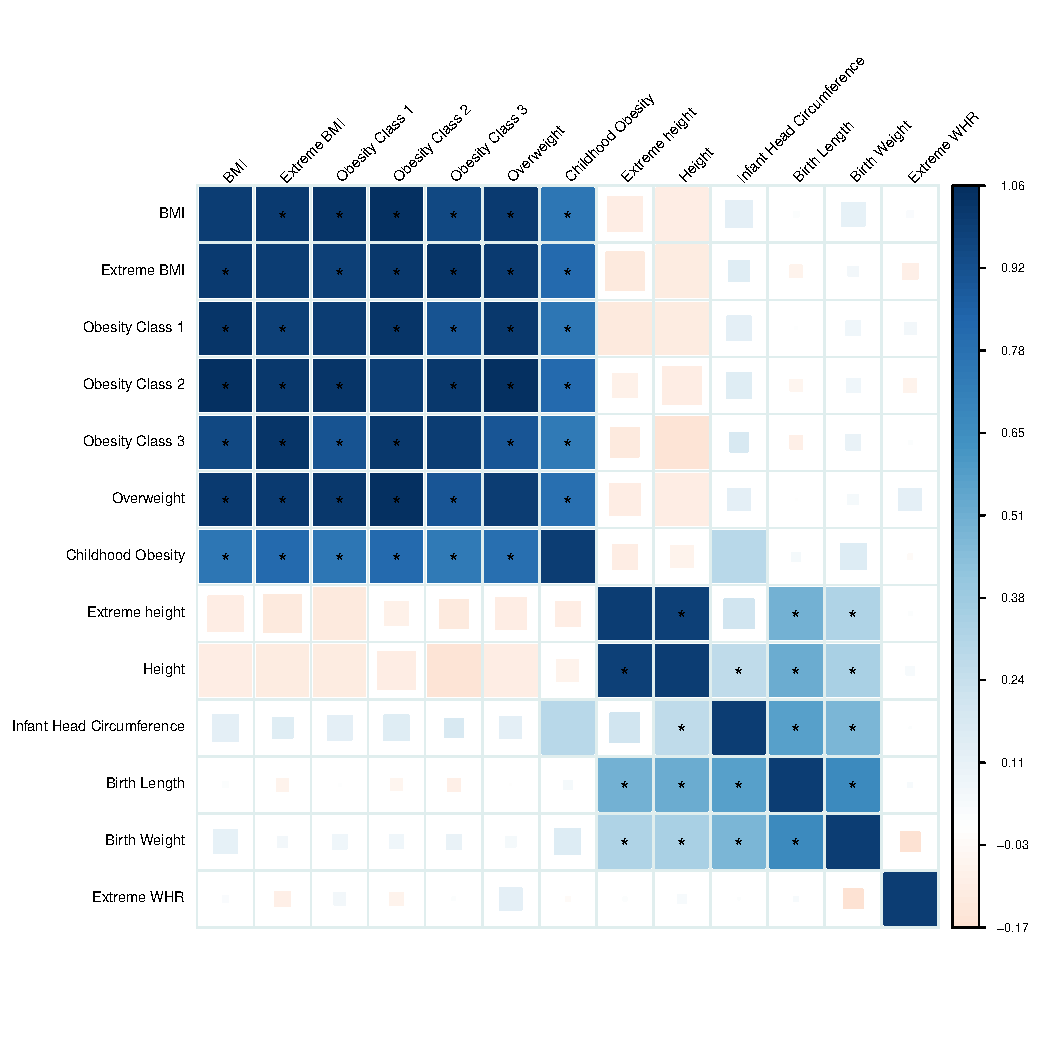
\includegraphics[scale=0.8]{figs/giant_supp.pdf}
\caption{\label{giant}\small{\textit{Genetic correlations among highly correlated anthropometric traits from studies by the GIANT and EGG consortia. The structure of the figure is the same as Figure \ref{Fig:300 Gencors} in the main text: 
blue corresponds to positive genetic correlations; red corresponds to negative genetic correlation. 
Larger squares correspond to more significant $p$-values.
Genetic correlations that are different from zero at 1\% FDR are displayed as full-sized squares. 
Genetic correlations that are significantly different from zero at significance level 0.05 after Bonferroni correction are given an asterisk.}}}
\end{centering}
\end{figure}
\newpage

\subsection*{Genetic Correlations among Smoking Traits}
\begin{figure}[!ht]
\begin{centering}
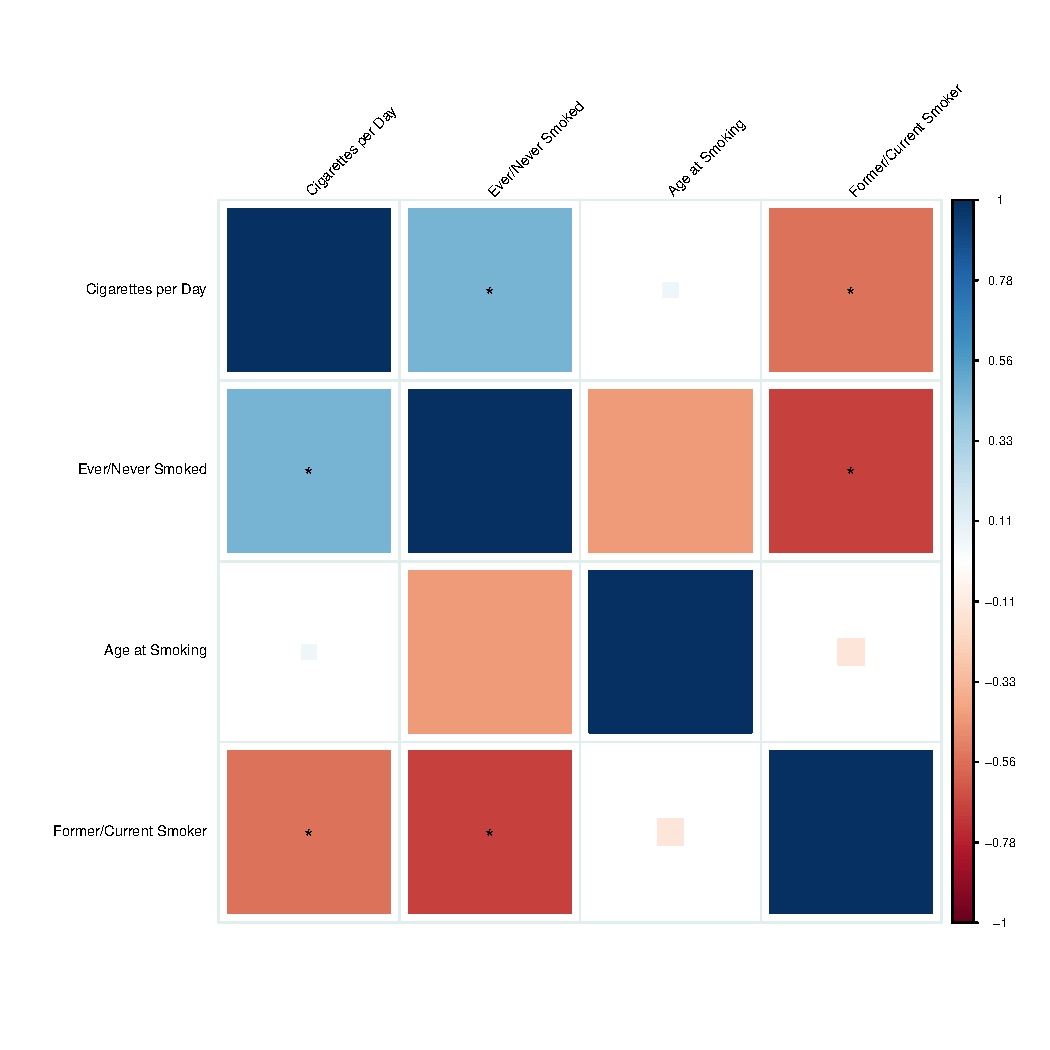
\includegraphics[scale=0.8]{figs/tag_supp.pdf}
\caption{\label{smoking}\small{\textit{Genetic correlations among highly correlated smoking-related traits from the Tobacco and Genetics (TAG) consortium. The structure of the figure is the same as Figure \ref{Fig:300 Gencors} in the main text: 
blue corresponds to positive genetic correlations; red corresponds to negative genetic correlation. 
Larger squares correspond to more significant $p$-values.
Genetic correlations that are different from zero at 1\% FDR are displayed as full-sized squares. 
Genetic correlations that are significantly different from zero at significance level 0.05 after Bonferroni correction are given an asterisk.}}}
\end{centering}
\end{figure}
\newpage

\subsection*{Genetic Correlations among Insulin-Related Traits}
\begin{figure}[!ht]
\begin{centering}
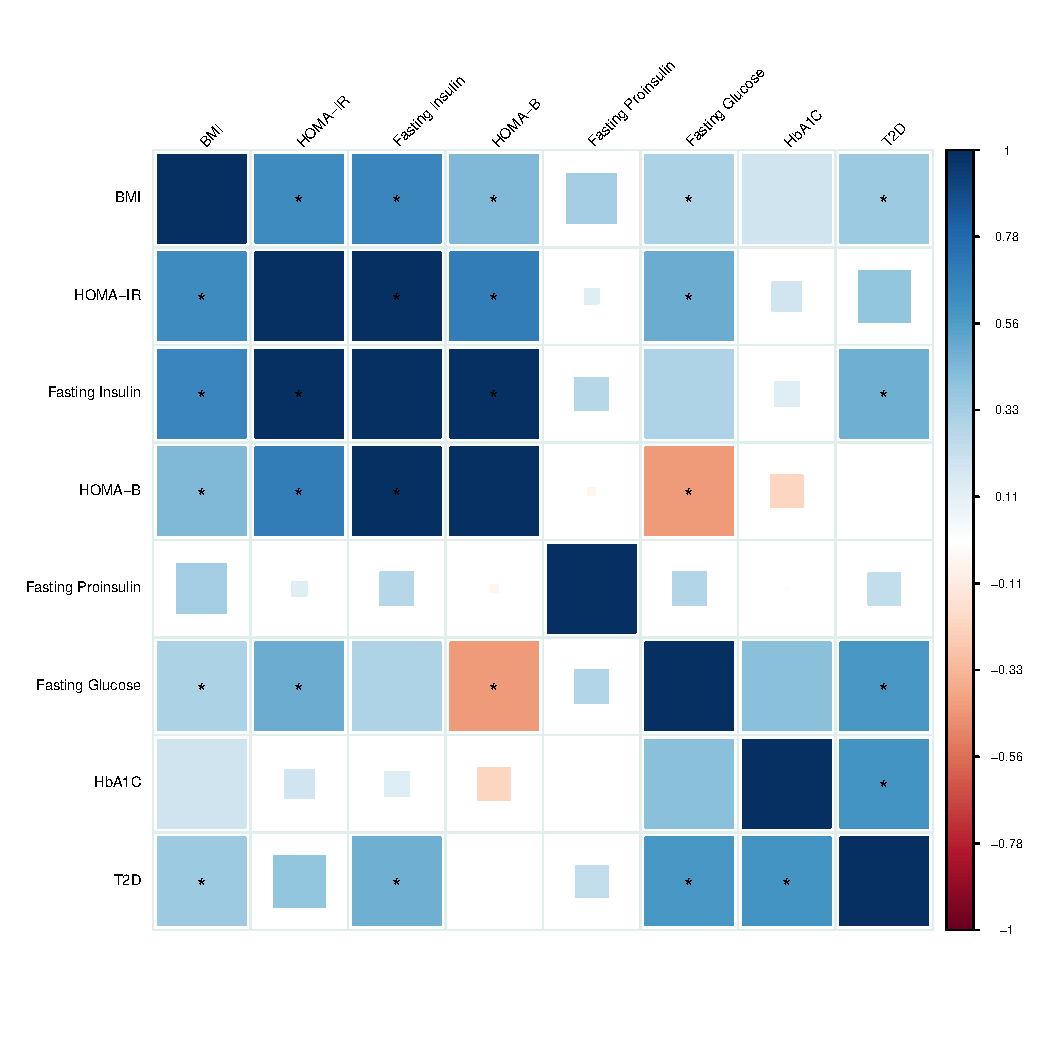
\includegraphics[scale=0.8]{figs/magic_supp.pdf}
\caption{\label{insulin}\small{\textit{Genetic correlations among highly correlated insulin-related traits from studies by the MAGIC consortium. The structure of the figure is the same as Figure \ref{Fig:300 Gencors} in the main text: 
blue corresponds to positive genetic correlations; red corresponds to negative genetic correlation. 
Larger squares correspond to more significant $p$-values.
Genetic correlations that are different from zero at 1\% FDR are displayed as full-sized squares. 
Genetic correlations that are significantly different from zero at significance level 0.05 after Bonferroni correction are given an asterisk.}}}
\end{centering}
\end{figure}
\newpage


\subsection*{Comparison of Metabolic Genetic Correlations from LDSC to Results from Vattikuti, et al}
\begin{figure}[!ht]
\begin{centering}
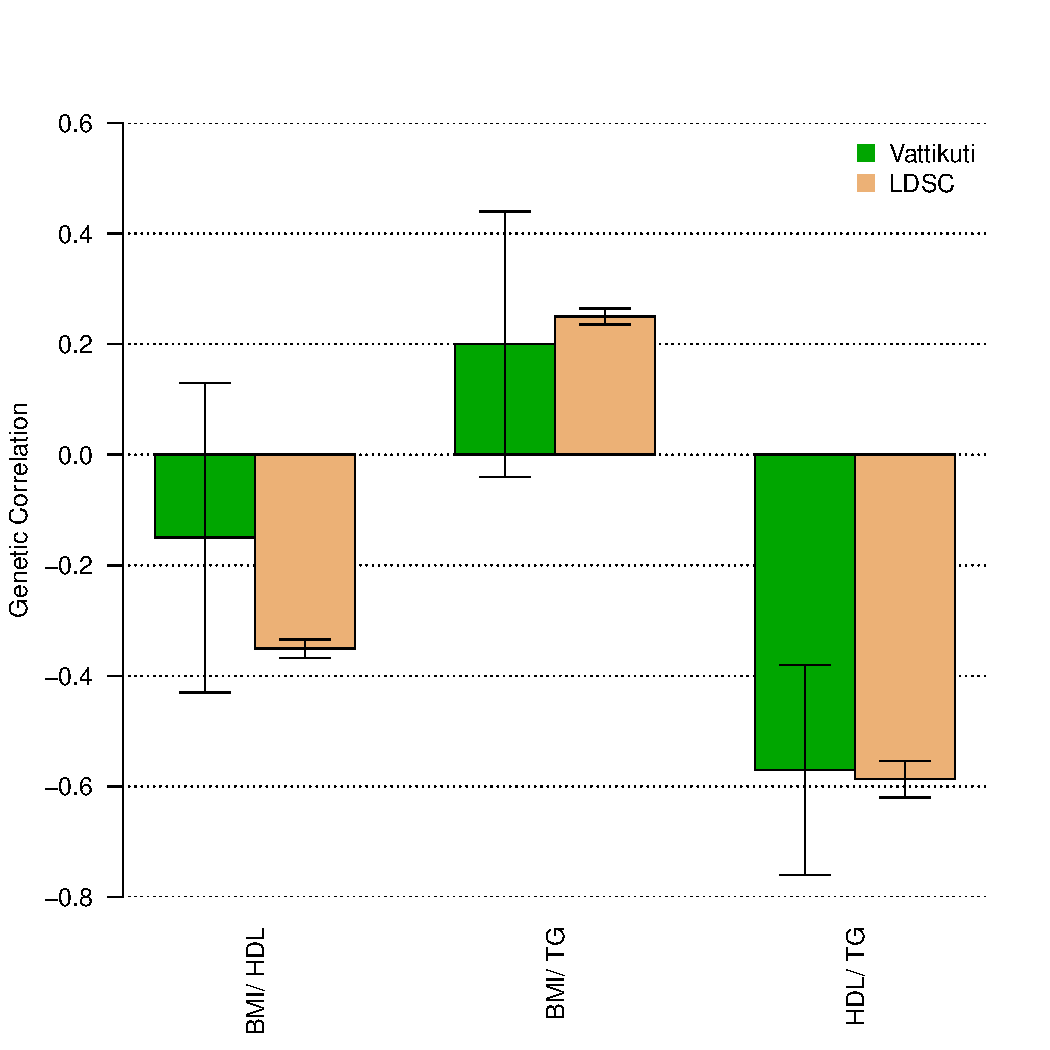
\includegraphics[scale=0.8]{figs/vattikuti.pdf}
\caption{\label{vattikuti}\small{\textit{This figure compares the estimates of genetic correlations between metabolic traits from table 3 of Vattikuti, et al. \cite{vattikuti2012heritability}
to the results obtained using LD Score regression (with much larger sample sizes) in this paper.}}}
\end{centering}
\end{figure}
\newpage

\subsection*{Schizophrenia / TG Conditional QQ Plot with and without the MHC}
\begin{figure}[!ht]
\begin{centering}
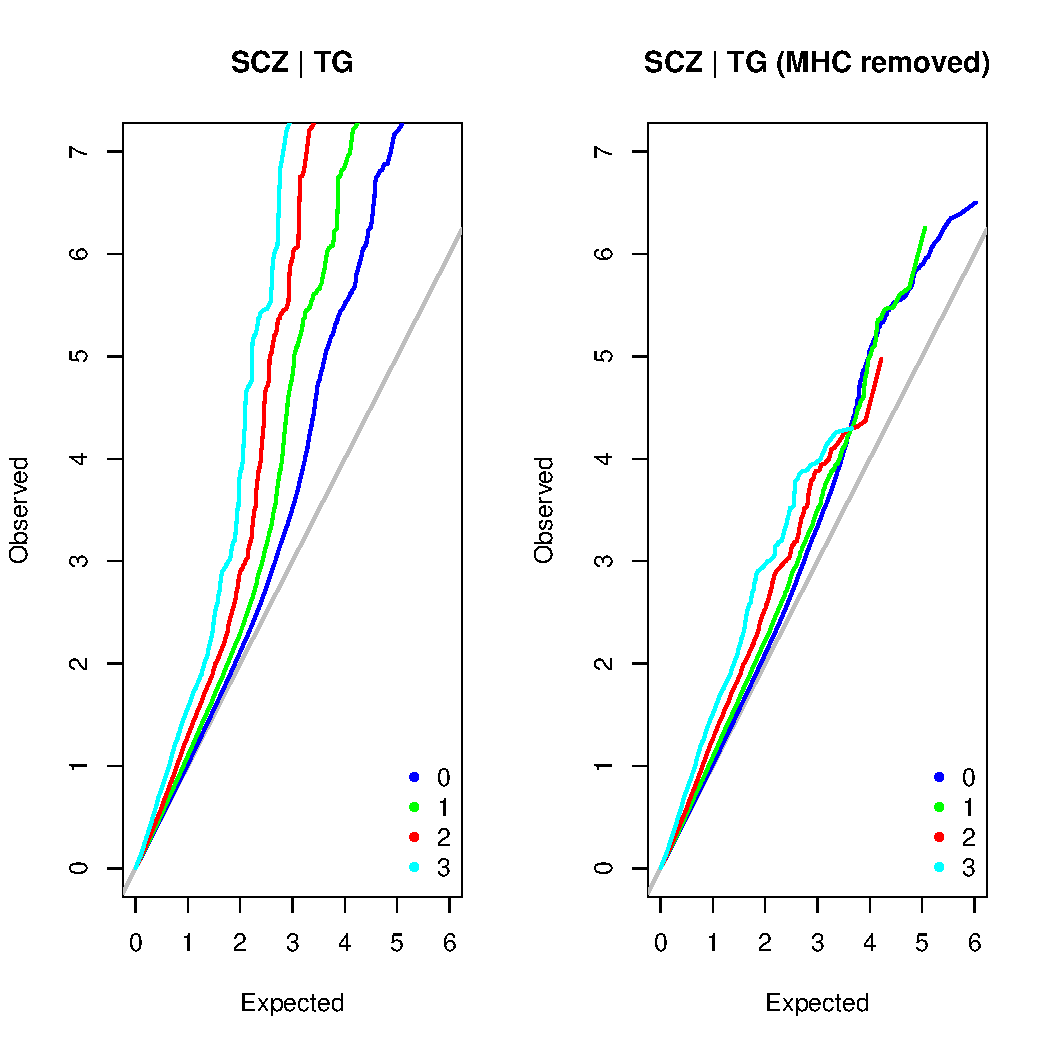
\includegraphics[scale=0.9]{figs/PGC1_pleiotropy_filter.png}
\caption{\label{qq_tg}\small{\textit{We reproduced the conditional QQ plot comparing schizophrenia (SCZ) and triglycerides (TG) from Andreassen et al. \cite{andreassen2013improved} (left). 
The major histocompatibility complex (MHC, approximately chr6, 25-35 MB) is
a genomic region featuring SNPs with exceptionally high LD Scores and the strongest GWAS association to schizophrenia.
Removing the MHC removes almost all signal from the conditional QQ plot (right), which is consistent with the 
near-zero genetic correlation between schizophrenia and TG estimated via LD Score regression.}}}
\end{centering}
\end{figure}
\newpage

%%%%%%%%%%%%%%%%%%%%%%%%%%%%%%%%%%%%%%%%%%%%%%%%%%%%%%%%%%%%%%%
\section*{Collaborators}
%%%%%%%%%%%%%%%%%%%%%%%%%%%%%%%%%%%%%%%%%%%%%%%%%%%%%%%%%%%%%%%


%%%%%%%%%%%%%%%%%%%%%%%%%%%%%%%%%%%%%%%%%%%%%%%%%%%%%%%%%%%%%%%
\section*{Supplementary References}
%%%%%%%%%%%%%%%%%%%%%%%%%%%%%%%%%%%%%%%%%%%%%%%%%%%%%%%%%%%%%%%

\end{document}
